% ===========================================================================
% Three Categories, One Waste Stream: Solid-Waste Disposal, Open Burning and
% Domestic Wastewater in Pakistan
%
% Target journal: Environmental Modelling & Software (Elsevier)
% Document class: elsarticle, 5p layout
% ===========================================================================

\documentclass[5p,times,authoryear]{elsarticle}

% ===========================================================================
% Shared preamble for every manuscript in this repository.
%
% Papers using it:
%   paper/            agriculture inventory
%   paper_nowcast/    agricultural nowcasting
%   paper_national/   the nine-sector national inventory
%   notes/<sector>/   one data note per non-agriculture sector
%
% It exists because paper/ and paper_nowcast/ began as copies of one another
% and had already drifted five lines apart before a third manuscript existed.
% Eleven copies would drift eleven ways, and a macro that renders differently
% in two papers is the kind of defect nobody notices until proof stage.
%
% \graphicspath is deliberately NOT set here - each manuscript sets its own
% after \input{...preamble}, because figures live beside the document.
% ===========================================================================

\usepackage[utf8]{inputenc}
\usepackage[T1]{fontenc}
\usepackage{amsmath,amssymb}
\usepackage{graphicx}
\usepackage{booktabs}
\usepackage{multirow}
\usepackage{siunitx}
\usepackage[colorlinks=true,citecolor=blue,linkcolor=blue,urlcolor=blue]{hyperref}
% Document-information metadata for every PDF in the bundle (the seventh review noted
% the shipped PDFs carried none). Documents that set their own \hypersetup{pdftitle=...}
% keep it - hyperref takes the LAST setting, and this shared block runs first. Full
% tagged-PDF (tagpdf / \DocumentMetadata) is deliberately not attempted here: the
% installed LaTeX toolchain's support is not uniform across sixteen documents, and a
% half-tagged bundle is worse than an honestly untagged one; deferred deliberately.
\hypersetup{
  pdfauthor={Rehan Ahmad, Pakistan Air Quality Initiative (PAQI)},
  pdfsubject={A reproducible ten-sector national greenhouse-gas inventory
              for Pakistan},
  pdfkeywords={Pakistan, greenhouse gas inventory, IPCC 2006 Guidelines, MRV,
               reproducible research, emissions, air pollutants},
}
\usepackage{caption}
\captionsetup[table]{position=below}
\usepackage{enumitem}
\usepackage{xcolor}
\usepackage{float}
\usepackage{placeins}
\usepackage{tabularx}
\usepackage{natbib}
\usepackage{tikz}
\usetikzlibrary{arrows.meta,positioning,fit,backgrounds}

\setlength{\emergencystretch}{3em}

% Looser float placement to prevent pile-up in two-column mode.
\renewcommand{\topfraction}{0.95}
\renewcommand{\bottomfraction}{0.85}
\renewcommand{\textfraction}{0.05}
\renewcommand{\floatpagefraction}{0.85}
\setcounter{topnumber}{4}
\setcounter{bottomnumber}{3}
\setcounter{totalnumber}{6}

% ---------------------------------------------------------------------------
% Custom shorthand: in macros.tex since the ESSD re-targeting, because the national
% article compiles under the Copernicus class and cannot take this preamble (the class
% loads its own packages) but needs exactly the same macros. This file inputs it so that
% every other manuscript keeps compiling unchanged.
%
% THREE relative paths, because \input resolves against the COMPILE DIRECTORY and not
% against this file, so the depth is a property of whoever is building:
%   ../paper_common      a manuscript compiled from one level down
%   ../../paper_common   papers/<sector>/ and notes/<sector>/
%   ../../../paper_common  paper_national/versions/<v>/, since the national paper was
%                          versioned - that move is what added this third arm, and the
%                          supplement failed with "../../paper_common/macros.tex not
%                          found" until it was here
% A fourth depth needs a fourth arm, which is the cost of keeping a bare `latexmk` in a
% manuscript directory working without a TEXINPUTS set for it.
% ---------------------------------------------------------------------------
\IfFileExists{../paper_common/macros.tex}%
  {\input{../paper_common/macros}}%
  {\IfFileExists{../../paper_common/macros.tex}%
    {% ===========================================================================
% paper_common/macros.tex - the shorthand every manuscript shares.
%
% Split from preamble.tex in the ESSD re-targeting: the national article now compiles
% under the Copernicus class, which loads its own packages and forbids most of what
% preamble.tex sets (geometry-like options, a second hyperref, placeins), but it needs
% exactly the same shorthand as the sector reports. The macros therefore live here, on
% their own, and preamble.tex inputs this file so that every other manuscript keeps
% compiling unchanged. A macro that renders differently in two documents is the defect
% this file exists to prevent; define it once.
%
% Requires: siunitx (for \DeclareSIUnit and \si) - the caller loads it.
% ===========================================================================

% Gas and pollutant names.
\newcommand{\COtwo}{CO\textsubscript{2}}
\newcommand{\COe}{CO\textsubscript{2}e}
\newcommand{\CHfour}{CH\textsubscript{4}}
\newcommand{\NtwoO}{N\textsubscript{2}O}
\newcommand{\NHthree}{NH\textsubscript{3}}
\newcommand{\NOx}{NO\textsubscript{x}}
\newcommand{\SOtwo}{SO\textsubscript{2}}
\newcommand{\PM}{PM\textsubscript{2.5}}
\newcommand{\MCF}{MCF}
\newcommand{\Mt}{\text{Mt~\COe}}
\newcommand{\tCha}{\si{\tonne\per\hectare}}
\newcommand{\AFOLU}{AFOLU}
\newcommand{\GLW}{GLW\,4}
\newcommand{\EFone}{EF\textsubscript{1}}

% siunitx: allow Mt, Tg, ha, head, yr, dB
\DeclareSIUnit{\head}{head}
\DeclareSIUnit{\yr}{yr}
\DeclareSIUnit{\dB}{dB}

% A file name is the one long unbreakable token these documents are full of -
% \texttt{waste\_air\_pollutants\_2024.csv} is wider than a two-column measure and TeX prints
% it past the margin rather than breaking it. Allowing a break AFTER each escaped underscore
% costs nothing and inserts no hyphen, which matters: a hyphenated file name is a wrong file
% name. This is one line because every such name in every document is written with \_.
\let\pkinvunderscore\_
\renewcommand{\_}{\pkinvunderscore\allowbreak}
}%
    {\input{../../../paper_common/macros}}}
% Long unbreakable strings - output filenames, module paths, URLs in \texttt - do not fit a
% two-column measure and TeX prints them past the margin rather than breaking them. Nothing
% read the log, so 47 of those overruns shipped across seven documents. Emergency stretch lets
% the paragraph loosen instead, and \texttt is taught to break at the punctuation these names
% actually contain.
\emergencystretch=6em


\graphicspath{{figures/}}

% ---------------------------------------------------------------------------
\journal{Environmental Modelling \& Software}
% ---------------------------------------------------------------------------

\begin{document}

\begin{frontmatter}

\title{PakEmis Sector Technical Note TN04\\[4pt]
Three Categories Partitioning One Waste Stream: Solid-Waste Disposal, Open Burning
and Domestic Wastewater Emissions for Pakistan}

\author[paqi]{Rehan Ahmad\corref{cor1}}
\ead{rehan@pakairquality.com}

\address[paqi]{Pakistan Air Quality Initiative (PAQI), Karachi, Pakistan}

\cortext[cor1]{Corresponding author}

% --- Abstract ---
\begin{abstract}
Pakistan's waste sector has no current national greenhouse-gas estimate built from Pakistani
activity data, and the international products that fill the gap disagree with each other by
amounts larger than the mitigation decisions they inform. We report the sector for
FY2023--24 at
\SI{37.45}{\mega\tonne} \COe{} (AR5, \SI{36.37}{\mega\tonne} on AR6) across three IPCC
categories: domestic wastewater (4D1) at \SI{24.46}{\mega\tonne}, solid-waste disposal (4A)
at \SI{9.17}{\mega\tonne} and open burning (4C2) at \SI{3.83}{\mega\tonne}. The current 10,000-draw conditional parameter ensemble gives \SIrange{25.4}{61.5}{\mega\tonne} CO$_2$e (2.5th--97.5th percentiles). It preserves the asymmetric effluent-N$_2$O factor treatment and the bounded waste-fate calculation; management alternatives and missing sources remain outside that interval. The same fate realisations support open-burning air pollutants, including \SI{63.85}{\kilo\tonne} primary PM$_{2.5}$, without double-counting generated material. The national annual core extends the disposal-history state and supported population inputs through FY2024--25; this note retains its detailed FY2023--24 analysis.

Two features distinguish the estimate from a conventional compilation. First, solid-waste
disposal and open burning are computed from one mass-balanced national waste-generation
figure rather than from separate literature: \SI{31.56}{\mega\tonne}
generated, \SI{50.3}{\percent} collected to disposal and the remainder uncollected, of which
\SI{60}{\percent} burns and the unburned \SI{6.27}{\mega\tonne} is carried as an explicit
unresolved fate with no emissions pathway applied.
Disposed plus uncollected equals generated, asserted with exact
equality rather than reconciled afterwards, so an argument about the collection rate moves
emissions between two categories without creating or destroying waste. Inventories that
estimate landfilling and open burning independently have no such constraint, and nothing then
forces their sum to be a quantity of waste the country actually produces.

Second, the largest category rests on an assumption the guidelines leave genuinely open for
Pakistani conditions. IPCC gives a methane correction factor of \num{0.5} for stagnant sewers
and \num{0.1} for discharge to a flowing river; Pakistani urban drainage has properties of
both. At \num{0.5} domestic wastewater is \SI{24.46}{\mega\tonne} and the sector sits at
\SI{141}{\percent} of EDGAR's year-matched Pakistani waste total; at \num{0.1} it is
\SI{15.39}{\mega\tonne} and the sector lands close to EDGAR. The physical description of the
drains supports the higher value and the only independent comparator supports the lower. We
report both, adopt \num{0.5} as central because the physical description is the stronger
evidence, and identify the measurement that would settle it: dissolved-methane sampling on
urban drains across a seasonal cycle. The physical description and the external inventory comparison play different roles; agreement with EDGAR is not used to select the central parameter. Seasonal measurements of drain methane could discriminate between the retained structural interpretations.

\end{abstract}

\begin{keyword}
municipal solid waste \sep first order decay \sep open burning \sep domestic wastewater \sep
methane correction factor \sep exhaustive partition \sep IPCC 2006 Guidelines \sep
Monte-Carlo uncertainty \sep Pakistan \sep MRV
\end{keyword}

\end{frontmatter}

%% Generated by scripts/make_release_cover.py; says which release this documents.
% The Sector Technical Note banner (v1.0.0). Each sector manuscript is a PakEmis Sector
% Technical Note, numbered TN01-TN10 in src/pkinv/release.py (TECHNICAL_NOTES), and says
% so on its first page: it documents ONE sector module of the release named in the block
% that follows, and the national totals are stated only in the data-description article
% (the cover block below reproduces them as release identity, not as a claim of this note).
% Usage, in the document body before the release cover:  \TNBanner{TN01}
\providecommand{\TNBanner}[1]{%
  \noindent\fbox{\parbox{\dimexpr\linewidth-2\fboxsep-2\fboxrule}{%
    \textbf{PakEmis Sector Technical Note #1.} Technical documentation of one sector
    module of the PakEmis release identified below, deposited with the data as part of the
    documentation record. The national data-description article (\texttt{paper\_national/})
    is the only document that states the national totals as its own result.%
    \InputIfFileExists{../../paper_common/generated_availability_tn}{}{}%
  }}\par\medskip}

\TNBanner{TN04}
%% GENERATED by scripts/make_release_cover.py from outputs/release_manifest.json.
%% Do not edit: the edit will be overwritten and CI diffs the result.
\newcommand{\ReleaseCover}{%
\begin{center}\small
\setlength{\fboxsep}{4pt}%
\fbox{\begin{minipage}{\dimexpr\linewidth-2\fboxsep-2\fboxrule\relax}\footnotesize
\textbf{Release provenance.} This document describes PakEmis under the period, configuration and source boundaries specified in its methods. The identifiers below link it to the accompanying products and source register.\\[2pt]
\begin{tabular}{@{}p{0.32\linewidth}@{\hspace{0.03\linewidth}}p{0.65\linewidth}@{}}
Release version & \texttt{1.0.0rc69} \\
Commit & \texttt{d8d874622f9a} \\
Reporting period & July 2015--June 2025 (ten fiscal years) (2015-07-01 to 2025-06-30) \\
Reference & S\_TAN (household survey; TAN nitrogen) \\
FY2023--24 total & 444.61 Mt \COe{} (AR5) under S\_TAN, the reference; 449.85 Mt under L\_TAN \\
Release manifest & \texttt{ac0ffe93ad9fcd88} (SHA-256 of \texttt{outputs/release\_manifest.json}, first 16) \\
Source manifest & \texttt{c1be6d314cfce1ea} (SHA-256 of \texttt{data/manifests/source\_manifest.csv}, first 16) \\
Data-description article & \texttt{paper\_national/} (ESSD, in preparation), same release
\end{tabular}
\end{minipage}}
\end{center}}

\ReleaseCover

% ---------------------------------------------------------------------------
% Main body
% ---------------------------------------------------------------------------

% ===========================================================================
\section{Introduction}
\label{sec:introduction}
% ===========================================================================

Waste is the category of a national greenhouse-gas inventory where the arithmetic is easiest
and the activity data hardest. The emission factors are few and well characterised; what is
difficult is knowing how much waste a country generates, what fraction of it reaches a
disposal site, what happens to the fraction that does not, and how the sewage of a large
population is actually handled. None of those quantities is metered anywhere in Pakistan.

That difficulty has a specific consequence for how the sector is usually compiled. Because the
activity data must be modelled rather than read, each category tends to be estimated on its
own terms: landfill methane from a tonnage assumption, open burning from a per-capita burning
rate in the literature, wastewater from a population and a default organic load. The three
estimates are then reported together. Nothing in that procedure requires the waste sent to
landfill and the waste openly burned to sum to a quantity of waste the country plausibly
produces, and in general they do not.

\subsection{What this paper does}

We report Pakistan's waste sector for FY2023--24 from Pakistani activity data, with the three
categories constructed so that the constraint the conventional procedure lacks is enforced by
construction. A single national waste-generation figure is partitioned: what is collected
goes to the first-order-decay model for solid-waste disposal, what is not collected is what
can burn, and the two sum to the generated quantity exactly. The partition is asserted in code
with equality rather than checked afterwards with a tolerance, because a tolerance permits
precisely the drift the constraint exists to remove.

The result is a sector total of \SI{37.45}{\mega\tonne} \COe{}, of which domestic wastewater
is two-thirds. It is the second most uncertain sector in the national inventory that contains
it, and this paper is as much about where that uncertainty lives and what would reduce it as
about the central estimate.

\subsection{Why Pakistan, and why this sector now}

Pakistan is the fifth most populous country in the world, urbanising rapidly, and its most
recent full national inventory submission reports for FY2017--18 \citep{pakbur1}. In the
interim the international gridded products---EDGAR \citep{edgar2025booklet,crippa2020} and Climate
TRACE \citep{climatetrace}---supply the numbers that inform policy. They are global models
applying globally consistent assumptions to nationally reported activity, which is their
strength for cross-country comparison and their limitation for any one country: where a
national compiler can consult a sanitation survey or a district population panel, a global
product must choose a default.

The waste sector is where that difference bites hardest, for two reasons. Its activity data
are the least standardised internationally, so the defaults do the most work. And it is
dominated by methane, whose short atmospheric lifetime makes it the gas where near-term
mitigation is most effective and therefore where the estimate most directly changes what a
government should do.

\subsection{Contributions}

\begin{enumerate}[leftmargin=*,itemsep=2pt,topsep=3pt]
\item \textbf{A current national waste-sector inventory for Pakistan} covering solid-waste
  disposal, open burning and domestic wastewater, from a district population panel and
  national sanitation statistics rather than from a global model's Pakistani slice.
\item \textbf{One waste stream, mass-balanced across its fates}: collected and uncollected
  shares sum to generation exactly, two fates carry emissions pathways (4A, 4C2) and the
  unburned remainder ships as an explicit unresolved row rather than a silent omission. The
  closed balance removes a class of inconsistency that independent estimation cannot
  detect (Section~\ref{sec:methods}).
\item \textbf{Both readings of the sewer methane correction factor}, with the evidence for
  each stated and neither resolved by fiat, together with the measurement that would settle
  it (Section~\ref{sec:discussion}).
\item \textbf{A spin-up sensitivity for the decay model}, quantifying how much of today's
  landfill methane comes from waste deposited before the activity panel begins---a question
  most first-order-decay implementations answer implicitly and do not report.
\item \textbf{An air-pollutant layer on the same activity basis} as the greenhouse gases, so
  that open burning's particulate can be compared with other Pakistani sources without the
  usual mismatched-activity problem.
\end{enumerate}

Method that this sector shares with the other nine of the national inventory---the module
contract, the uncertainty treatment, the notation keys, the accounting closures---is
documented in the national manuscript \citep{ahmad2026national} and not repeated here.

% ===========================================================================
\section{Related Work}
\label{sec:related}
% ===========================================================================

\subsection{Global products and what they can and cannot resolve}

EDGAR \citep{edgar2025booklet,crippa2020} reports a Pakistani waste total covering disposal, burning
and wastewater together, and is the closest external comparator to the scope reported here.
Climate TRACE \citep{climatetrace} takes a different approach, inferring emissions from
asset-level and remote-sensing evidence. Both are global products: they apply a consistent
methodology across every country, which is what makes them comparable and also what limits
them nationally. A global waste model must assume a collection rate and a sewer condition for
Pakistan; a national compiler can consult the sanitation statistics and the district
population panel that describe it.

The disagreement between products is not a defect of any of them, but it is large enough to
matter. This inventory sits at \SI{141}{\percent} of EDGAR's year-matched Pakistani waste
figure, and
Section~\ref{sec:validation} argues that a single assumption---the sewer methane correction
factor---accounts for most of the difference.

\subsection{Waste generation and composition in South Asia}

Per-capita waste generation and its composition are the two activity inputs the sector cannot
avoid, and both are surveyed rather than metered. The global compilation by
\citet{kaza2018} is the standard reference; its Pakistan generation row re-bins the one
primary national survey, the Pak-EPA eight-city study \citep{pakepa1996}, whose rates are
used here directly, and its collection coverage supplies the uncollected fractions.
Composition matters more than it first appears: the fossil carbon fraction of municipal
waste---plastics, textiles, rubber---determines how much of the \COtwo{} from open burning is
reportable, because the biogenic remainder is a memo item under IPCC's convention rather than
a national-total emission.

\subsection{First Order Decay and its implementation choices}

Landfill methane is not a function of this year's waste but of every year's waste still
decaying, which is why IPCC's Volume~5 method is a first-order decay model over a deposit
history rather than an emission factor applied to an annual tonnage. Three implementation
choices then do most of the work and are reported inconsistently in the literature: the decay
constant, the methane correction factor describing site management, and how far back the
deposit series is extended before the model is considered spun up.

The third is the one this paper treats explicitly. A model started at the first year of an
activity panel implicitly asserts that nothing was landfilled before it, which is never true
and always biases the estimate low. The size of that bias is rarely reported.
Section~\ref{sec:results} reports it here.

\subsection{The wastewater methane correction factor}

For domestic wastewater the corresponding controversy is the methane correction factor, which
translates a sanitation pathway into the fraction of its organic load that degrades
anaerobically. IPCC's default table distinguishes stagnant sewers from flowing ones by an
order of magnitude in that fraction, and the distinction was drawn for systems that are
clearly one or the other. Open urban drains that are stagnant in the dry season and flowing
after rain, and which discharge to irrigation channels, are not obviously either.

Pakistani sanitation coverage itself is well characterised: the WHO/UNICEF Joint Monitoring
Programme \citep{jmp2023} reports the population shares using sewers, septic systems, latrines
and open defecation, and those shares are what allocate the national organic load across
pathways here.
What the JMP does not report, and no Pakistani source does, is the hydraulic condition of the
sewered fraction---which is the quantity the correction factor is asking about.

% ===========================================================================
\section{Study Area and Data}
\label{sec:data}
% ===========================================================================

\subsection{Population, which is the activity datum}

Every category in this sector is driven by population. Waste generation is a per-capita rate
applied to urban and rural residents; the organic load entering the wastewater system is a
per-capita BOD applied to the same population split by sanitation pathway. There is no
tonnage measurement and no metered flow anywhere in the chain, so the population panel is the
activity data in a way that is unusual for an emissions inventory.

The panel is built at district level and interpolated between censuses, covering
\num{134} districts, with the 2023 census as its reference---the census's full frame
including the Islamabad Capital Territory, Gilgit-Baltistan and Azad Kashmir, a
deliberately wider base than the \num{116} four-province districts the agriculture
sector allocates to, whose activity statistics are provincial in scope. It resolves to
\SI{97}{} million urban and \SI{150}{} million rural residents, \SI{247}{} million in total.
The urban/rural split is load-bearing twice over: urban residents generate more waste per head
and are far more likely to have their waste collected, and the two effects run in opposite
directions for emissions, since collected waste goes to a decaying landfill while uncollected
waste burns.

Building the panel at district level rather than nationally is what makes the provincial
allocation in Section~\ref{sec:results} a real geography rather than a national figure split
by a population share, and it is the same panel that drives the sector's air-pollutant layer.

\subsection{Waste generation and collection}

Per-capita generation is \SI{0.453}{\kilo\gram} per person per day urban and
\SI{0.283}{\kilo\gram} rural, from the Pak-EPA eight-city survey \citep{pakepa1996}, the
rates the \citet{kaza2018} Pakistan row re-bins. Across the panel that is
\SI{31.56}{\mega\tonne} of municipal solid waste a year.

Collection is expressed as its complement, the uncollected fraction: \SI{30}{\percent} urban
and \SI{70}{\percent} rural, which resolves to \SI{50.3}{\percent} of national generation
collected. Of the uncollected remainder, \SI{60}{\percent} is openly burned; the rest is
dumped, tipped into watercourses or otherwise disposed of without combustion and emits nothing
this category reports.

These three parameters---two generation rates, two uncollected fractions and one burned
fraction---are the softest inputs in the sector, and Section~\ref{sec:limitations} says so.
They are also the only place where a judgement moves emissions \emph{between} categories
rather than changing the total, which is a property of the partition rather than of the
parameters.

\subsection{Waste composition}

Open burning needs the carbon content of what burns. Dry matter is \SI{70}{\percent} of wet
weight; total carbon is \SI{0.2195}{\tonne} per wet tonne and the fossil fraction of it is
\SI{0.0757}{\tonne} per wet tonne, so roughly a third of the carbon in Pakistani municipal
waste is fossil in origin. That third is what produces reportable \COtwo{}; the biogenic
remainder is a memo item, following IPCC Volume~5 Chapter~5 \S5.1.

\subsection{Sanitation}

The wastewater category needs the population split across sanitation pathways, because the
methane correction factor is a property of the pathway rather than of the person. Shares come
from the WHO/UNICEF Joint Monitoring Programme \citep{jmp2023}, each year taking its own:
sewered, septic, latrine and open defecation,
each carrying its own correction factor (\num{0.5}, \num{0.5}, \num{0.1} and \num{0}
respectively).

Organic load is \SI{40}{} g BOD per person per day, the regional default covering Pakistan,
with an industrial-and-commercial correction of \num{1.25} for load discharged to the domestic
system from small commercial premises. Nitrous oxide is computed from protein consumption
rather than from BOD, which is why it is invariant under both of the sensitivities reported
in Section~\ref{sec:results}.

\subsection{What this inventory has not obtained, and what it would change}

Nothing compiled here reports landfill tonnages at facility level, methane recovery at any
site, industrial solid-waste quantities, or industrial wastewater organic loading. Three of
those four have leads that have not been followed: the Urban Unit has mapped solid-waste
services and facilities across Punjab's tehsils, PBS's district-level living-standards survey
records household disposal route---municipal collection, private, public bins, roadside,
waterway, open space---and PCRWR has published organic loading for named Pakistani drains.
None would give complete national coverage, and each would replace a national assumption with
district or facility evidence for the population it covers. The first two
would replace modelled disposal with measured disposal; the second two are whole categories
this inventory reports as not estimated. Section~\ref{sec:limitations} takes each in turn.

% ===========================================================================
\section{Methods}
\label{sec:methods}
% ===========================================================================

\subsection{One generation figure, mass-balanced across fates}
\label{sec:partition}

The sector's structure follows from a single decision: municipal solid waste is one national
quantity that must be divided, not three quantities to be estimated separately.

Annual generation is
\begin{equation}
G \;=\; 365 \sum_{d} \left( P^{u}_{d} g_{u} + P^{r}_{d} g_{r} \right),
\end{equation}
over districts $d$, with $g_u$ and $g_r$ the urban and rural per-capita rates. The collected
fraction, which is what reaches a disposal site,
\begin{equation}
D \;=\; 365 \sum_{d} \left( P^{u}_{d} g_{u} (1 - u_{u}) + P^{r}_{d} g_{r} (1 - u_{r}) \right),
\end{equation}
uses the uncollected fractions $u_u$ and $u_r$, and the uncollected remainder is $U = G - D$
by construction rather than by a second estimate. Of that remainder, the burned quantity is
$B = f_b U$.

The identity $D + U = G$ is asserted in code with exact equality, and a test fails if it ever
ceases to hold. (Tier status is stated per component rather than per sector, in
\ref{app:tiers}: the categories share one country-specific activity basis but differ in how
much of each calculation is a default.) This is the property that separate estimation cannot provide. If landfill
tonnage comes from one source and open-burning tonnage from another, their sum is unconstrained
and can exceed or fall short of national generation without anything in the calculation
noticing; here, an argument about the collection rate moves emissions between 4A and 4C2 and
changes the total only through the different methane yields of the two fates.

For FY2023--24 this gives \SI{31.56}{\mega\tonne} generated, \SI{15.88}{\mega\tonne} collected to
disposal, \SI{15.67}{\mega\tonne} uncollected and \SI{9.40}{\mega\tonne} openly burned. The
partition is published as an executable fate ledger
(\texttt{outputs/waste\_ledger\_2024.csv}, the same claimant structure as the transport fuel
ledger), whose writer raises if either tier fails to close and whose final row is the fate
this inventory does not model: \SI{6.27}{\mega\tonne} of uncollected waste that does not
burn---dumped on land or tipped into watercourses, carried explicitly rather than silently.

\subsection{Solid-waste disposal: First Order Decay (4A)}

Methane from a disposal site in year $t$ depends on every year's deposit still decaying, so
IPCC Volume~5 Chapter~3's first-order decay model is run over a deposit history rather than
applied to a single year's tonnage. Decomposable degradable organic carbon accumulates and
decays as
\begin{align}
\mathrm{DDOCm}_{a}(t) &= W(t)\,\mathrm{DOC}\cdot\mathrm{DOC_f}\cdot\mathrm{MCF}
   + \mathrm{DDOCm}_{a}(t{-}1)\,e^{-k}, \\
\mathrm{CH_4}(t) &= \left[\mathrm{DDOCm}_{a}(t{-}1)\left(1 - e^{-k}\right)\right] F
   \cdot \tfrac{16}{12},
\end{align}
with $k = \num{0.065}$, $\mathrm{DOC_f} = \num{0.5}$, $\mathrm{MCF} = \num{0.6}$ and
$F = \num{0.5}$.

Two parameters are deliberately zero. No methane recovery is credited, because none is
documented at national scale and crediting an undocumented recovery would understate the
category. The oxidation factor is zero for the same class of reason: IPCC's non-zero oxidation
applies to managed sites with a cover layer, and Pakistani disposal is predominantly
unmanaged, where the thin intermittent cover that drives oxidation is absent.

\subsubsection{Spin-up, and why it is reported rather than assumed}

The activity panel begins in 2000, but waste deposited before then is still emitting. Starting
the model at the panel's first year with an empty site would assert that Pakistan landfilled
nothing before 2000, which is false and biases the estimate low.

The deposit series is therefore back-projected to 1960 at \SI{40}{\percent} of the panel's
first-year tonnage, and the model is run from there. Because that back-projection is an
assumption rather than data, the sector reports what it is worth: without spin-up the category
would be \SI{8.07}{\mega\tonne} instead of \SI{9.17}{\mega\tonne}, so pre-2000 deposits
contribute \SI{12}{\percent} of today's landfill methane. A reader who prefers to start at the
panel can read the alternative directly from the output file rather than recomputing it.

\subsubsection{The monthly state engine, and why it is one recursion}

The national release resolves the disposal stream into fiscal months, and the
engine behind those months is this model run at a monthly step rather than a
reshaped annual answer: one continuous single-pool recursion from the 1960
spin-up, $S_m = S_{m-1}\,e^{-k\,d_m/365.25} + W_m$, where $d_m$ is the month's
exact calendar length (leap Februaries included) and $W_m$ deposits the month's
own calendar year's tonnage, days-weighted within the year. Running one recursion
rather than a per-year replay matters for three named reasons: state flows across
fiscal boundaries (June's stock is July's opening balance, so no seam appears at
the year change); each month deposits its \emph{own} year's waste (a per-year
replay had injected the panel's maximum year into every year's stock); and the
reaction delay between deposit and the onset of decay is a declared parameter
(\texttt{swds\_delay\_months}, the IPCC six-month convention) applied as a shape
refinement only. The single pool is kept deliberately --- the annual model carries
one decay constant, and a cohort structure would claim a waste-composition split
no Pakistani record supports. The annual control is preserved exactly by
construction: each fiscal year's twelve shares are normalised against its own
annual figure, so the monthly engine decides only \emph{when} within the year,
never how much, and the within-year spread it computes is printed into the
month rows' basis rather than asserted in prose.

\subsection{Open burning (4C2)}

IPCC Equation~5.1 applied to the burned quantity $B$, taking that chapter's own
allowance to combine the dry-matter, carbon-content and fossil-fraction terms into one
coefficient rather than carrying them separately:
\begin{equation}
\mathrm{CO_2} \;=\; B \cdot \mathrm{CF_{fossil}} \cdot \mathrm{OF}
  \cdot \tfrac{44}{12},
\end{equation}
where $\mathrm{CF_{fossil}}$ is the fossil carbon per \emph{wet} tonne given in
Section~\ref{sec:data} and the oxidation factor is $\mathrm{OF} = \num{0.71}$. Dry matter
does not appear here because it is already inside that coefficient; it enters this category
only through the \NtwoO{} factor, which IPCC states per dry tonne. The burned quantity $B$
is itself IPCC Equation~5.7.

Only the fossil carbon fraction produces reportable \COtwo{}. The biogenic fraction is
reported as a memo item at \SI{3520}{\giga\gram} \COtwo{}, outside the national total, because
that carbon was fixed from the atmosphere within the year. Methane and nitrous oxide from the
same burning \emph{are} counted regardless of carbon origin: incomplete combustion is a net
source however the carbon entered the waste stream.

\subsection{Domestic wastewater (4D1)}

Tier~1 over the sanitation-resolved population. Total organically degradable material is
\begin{equation}
\mathrm{TOW} \;=\; P \cdot \mathrm{BOD} \cdot 365 \cdot I,
\end{equation}
with $I = \num{1.25}$ the industrial-and-commercial correction, and methane is
\begin{equation}
\mathrm{CH_4} \;=\; \sum_{j} \mathrm{TOW}_{j} \cdot B_{0} \cdot \mathrm{MCF}_{j},
\end{equation}
summed over sanitation pathways $j$ with $B_0 = \SI{0.6}{\kilo\gram}$ \CHfour{} per kilogram
BOD. The pathway correction factors are the subject of Section~\ref{sec:discussion}.

Nitrous oxide is computed from protein consumption rather than from BOD, by the method of
the 2019 Refinement (Volume~5 Chapter~6, Equations~6.7 to 6.10a) \citep{ipcc2019}. Protein
supply is reduced to protein consumed (a factor of \num{0.96}) and its nitrogen (\num{0.16})
is allocated to the same sanitation pathways the methane uses, with factors of \num{1.1} for
household products, \num{1.1} for non-consumed protein (the chapter's updated Table~6.11,
taken over its text, which gives no increment where food waste goes with solid waste) and,
for industrial and commercial co-discharge, \num{1.25} on the sewered population only.
Treatment removes part of each pathway's nitrogen before discharge---\num{0.15} in septic
tanks, \num{0.12} in latrines and \num{0.40} in the treated share of sewered flow, which is
declared at \SI{1}{\percent} and not measured---and the nitrogen entering a treatment plant
emits there at \num{0.016}. What is left is summed over every pathway and emits at the
effluent factor of \num{0.005}; the whole population stays in the estimate. The result is
\SI{9.71}{\giga\gram} of \NtwoO{}. The single equation of the 2006 Guidelines, which this
inventory used before and which treats one nitrogen total on protein supply as effluent,
is retained as the alternative and gives \SI{11.45}{\giga\gram}. Neither method reads BOD or
the sewer correction factor. This is why nitrous oxide does not move under either of the
sensitivities reported below, and why a sensitivity row that reported methane alone would be
misread as a category total---a distinction this sector's output file previously got wrong
and now states explicitly.

% ===========================================================================
\section{Emission Factors and Parameters}
\label{sec:factors}
% ===========================================================================

Every factor and parameter used here is an IPCC 2006 default, a 2019 Refinement default
(the wastewater nitrous oxide chain) or a documented regional value,
with its source recorded in the versioned parameter table. Three deserve discussion because
the choice was not automatic.

\begin{table}[htbp]
\centering
\footnotesize
\begin{tabular}{@{}llr@{}}
\toprule
\textbf{Parameter} & \textbf{Applies to} & \textbf{Value} \\
\midrule
Generation rate, urban    & 4A, 4C2 & \SI{0.453}{} kg/cap/day \\
Generation rate, rural    & 4A, 4C2 & \SI{0.283}{} kg/cap/day \\
Uncollected fraction, urban & 4A, 4C2 & 0.30 \\
Uncollected fraction, rural & 4A, 4C2 & 0.70 \\
Burned fraction of uncollected & 4C2 & 0.60 \\
\midrule
Decay constant $k$        & 4A  & 0.065 yr$^{-1}$ \\
$\mathrm{DOC_f}$          & 4A  & 0.50 \\
MCF (site management)     & 4A  & 0.60 \\
$F$ (\CHfour{} in landfill gas) & 4A & 0.50 \\
Oxidation factor          & 4A  & 0 \\
Methane recovery          & 4A  & 0 \\
Back-projection to 1960   & 4A  & 40\% of first panel year \\
\midrule
Dry matter                & 4C2 & 0.70 \\
Total carbon              & 4C2 & \SI{0.2195}{} t C/t wet \\
Fossil carbon             & 4C2 & \SI{0.0757}{} t C/t wet \\
Oxidation factor          & 4C2 & 0.71 \\
\midrule
BOD                       & 4D1 & \SI{40}{} g/cap/day \\
$B_0$                     & 4D1 & \SI{0.6}{} kg \CHfour{}/kg BOD \\
MCF, sewered / septic     & 4D1 & 0.50 \\
MCF, latrine / open       & 4D1 & 0.10 / 0 \\
Industrial-commercial correction & 4D1 & 1.25 \\
\bottomrule
\end{tabular}
\caption{Parameters, with the IPCC volume and table recorded against each in
\texttt{data/waste\_params.csv}. The two zeros in the 4A block are deliberate and argued in
Section~\ref{sec:methods}, not defaults left unset. Full row-level provenance---value,
uncertainty, source and basis for every parameter and factor---is the generated table in
\ref{app:factors}.}
\label{tab:params}
\end{table}

\subsection{Two oxidation factors that must not be reconciled}

This sector carries an oxidation factor of \num{0.71} for open burning and \num{0} for
landfill, while the fossil-fuel sectors of the same inventory carry none at all. That looks
like an inconsistency and is not.

The 2006 Guidelines fold complete oxidation into the fuel combustion emission factors
themselves---Table~1.4 carries an explicit oxidation column of \num{1.0} for every fuel---so
applying the 1996-vintage \num{0.98} on top of a 2006 factor double-discounts. Open burning is
different in kind: it genuinely is incomplete, and \num{0.71} is the 2006 value that says so.
Landfill oxidation is different again, describing methane oxidised while passing through a
cover layer, which unmanaged Pakistani sites largely do not have.

Three different numbers describing three different physical situations. Tests pin all three,
so that a future reader who notices the apparent inconsistency and "corrects" it fails the
build rather than silently changing the sector.

\subsection{Fossil carbon, and why only a third of the burning \COtwo{} is reported}

Total carbon in Pakistani municipal waste is \SI{0.2195}{\tonne} per wet tonne, of which
\SI{0.0757}{\tonne}---roughly a third---is fossil. Only that third produces reportable
\COtwo{}; the rest was fixed from the atmosphere by plants within the year and is reported as
a memo item at \SI{3520}{\giga\gram}.

This convention is easy to apply inconsistently, because the same waste produces \CHfour{} and
\NtwoO{} that \emph{are} counted in full regardless of carbon origin. The distinction is not
about the waste but about the atmosphere: biogenic \COtwo{} returns carbon that was recently
removed, while methane from the same carbon is a different molecule with a different radiative
effect and no such offset.

\subsection{What the parameters are worth}

Three of the parameters above dominate the sector's uncertainty, and each is examined as a
published sensitivity rather than left implicit: the sewer MCF (Section~\ref{sec:discussion}),
the BOD rate, and the spin-up back-projection. The generation and collection rates are not
among them---not because they are well known, but because the partition means they move
emissions between categories more than they move the total.

\FloatBarrier
% ===========================================================================
\section{Validation}
\label{sec:validation}
% ===========================================================================

There is nothing to validate this sector against directly. No Pakistani facility reports
landfill gas, no drain is monitored for dissolved methane, and no survey measures how much
uncollected waste burns. What exists is other people's models, and comparing a model against a
model establishes consistency rather than accuracy. This section says what that comparison
does and does not show.

\subsection{Against EDGAR}

EDGAR reports Pakistani waste---disposal, burning and wastewater together---at
\SI{26.57}{\mega\tonne} \COe{} for 2023, year-matched to this inventory's reference year
\citep{edgar2025booklet}. This inventory reports \SI{37.45}{\mega\tonne}, or
\SI{141}{\percent} of it. (EDGAR's 2024 value, \SI{27.21}{\mega\tonne}, is carried in the
benchmark file for release-vintage context and is not the comparison basis.)

That row has changed sides during this work, which is what makes it informative. Before
domestic wastewater was built, this sector covered disposal and burning only and read
\SI{49}{\percent} of EDGAR; the gap was then a measure of what the missing category would add.
With 4D1 in, the sector overshoots. The same comparison has therefore diagnosed an omission
and then a possible overestimate, which is more than a single ratio usually earns.

The likeliest single cause is the sewer methane correction factor. At IPCC's stagnant-sewer
\num{0.5} the wastewater category is \SI{24.46}{\mega\tonne} and the sector overshoots; at the
river-discharge \num{0.1} it is \SI{15.39}{\mega\tonne}, the sector is
\SI{28.38}{\mega\tonne}, and the comparison lands at \num{1.07} times EDGAR. No other single
parameter in the sector can move it that far.

It would be easy to treat that as confirmation and adopt \num{0.1}. We do not, and
Section~\ref{sec:discussion} argues why: EDGAR is itself a model making its own assumption
about the same unmeasured quantity, so agreement between the two would demonstrate that two
models had made the same choice rather than that the choice is right.

\subsection{Against Climate TRACE}

Climate TRACE's Pakistani waste subsectors are built from a different evidence base again,
including facility detection. Its solid-waste figures are broadly consistent with the disposal
category reported here; its coverage of open burning and domestic wastewater is not
constructed on a comparable scope, so a total-to-total comparison would mislead rather than
inform and is not reported as one.

\subsection{Against household survey evidence}

The 2024--25 Household Integrated Economic Survey asks every sampled household how its
waste is collected or disposed of \citep{hies2025}, and its design-weighted answers are the
first Pakistani survey evidence bearing on the partition's load-bearing parameters. They
disagree with the What a Waste collection coverage the partition is built on, in one
direction: \SI{42.0}{\percent} of urban households report no collection of any kind against
the \SI{30}{\percent} assumed, and \SI{93.4}{\percent} of rural households against
\SI{70}{\percent}. The route detail supports the open-dumping reading of the uncollected
stream---\SI{88.5}{\percent} of rural households report disposal to open space, and under
\SI{1}{\percent} to waterways.

Two caveats keep this a comparison rather than a correction. Household route shares are not
waste-mass shares: the survey weights households, not tonnes, and converting one to the
other needs stratum generation rates it does not carry. And counting public-bin use as
collected overstates collection where bins are cleared infrequently, which the same module
records. The configuration is therefore priced as a named structural scenario in the
supplement rather than adopted; because the partition conserves generated waste, moving the
uncollected fractions to the survey values moves emissions from slow landfill decay to
immediate burning without changing the waste the country produces.

\subsection{Internal checks that do have teeth}

Three checks are enforced on every run and, unlike the external comparisons, can fail.

\textbf{The mass balance closes.} Disposed plus uncollected equals generated, exactly.
This cannot detect a wrong collection rate, but it can and does detect the class of error
where a change to one category silently fails to appear in the other.

\textbf{The burned quantity is exactly the burned fraction of the uncollected remainder.}
Asserted with equality against an independently recomputed value, so a future refactor that
accidentally applies the burned fraction to total generation rather than to the uncollected
part fails immediately. That specific error would inflate open burning by a factor of two and
is entirely plausible.

\textbf{Provincial allocation reconciles exactly.} The four provinces and the territories sum
to the national figure for each category, not merely for the sector.

\subsection{What would constitute real validation}

Three measurements, in order of what they would settle. Dissolved-methane and flux sampling on
urban drains across a seasonal cycle would resolve the correction factor that dominates the
sector. Landfill gas monitoring at two or three large sites would test the first-order-decay
parameters directly. A waste-characterisation survey at the same sites would replace the
regional composition figures with Pakistani ones and firm up the fossil carbon fraction that
governs reportable \COtwo{} from burning.

None is expensive relative to what the sector contributes to national uncertainty. That
argument is made quantitatively in Section~\ref{sec:discussion}.

% ===========================================================================
\section{Results}
\label{sec:results}
% ===========================================================================

\subsection{The sector}

Pakistan's waste sector emitted \SI{37.45}{\mega\tonne} \COe{} in FY2023--24 on AR5 metrics, or
\SI{36.37}{\mega\tonne} on AR6. Domestic wastewater is \SI{65.3}{\percent} of it.

\begin{table}[htbp]
\centering
\footnotesize
\begin{tabular}{@{}llrrr@{}}
\toprule
\textbf{Category} & \textbf{Gas} & \textbf{Gg} & \textbf{Mt \COe{}} & \textbf{$\pm$\%} \\
\midrule
Open burning (4C2)        & \COtwo{} (fossil) & 1853.21 & 1.853 &  84.3 \\
                          & \CHfour{}         &   61.12 & 1.712 &  92.9 \\
                          & \NtwoO{}          &    0.99 & 0.262 & 124.2 \\
Solid-waste disposal (4A) & \CHfour{}         &  327.45 & 9.169 &  79.8 \\
Domestic wastewater (4D1) & \CHfour{}         &  781.63 & 21.886 & 73.7 \\
                          & \NtwoO{}          &    9.71 & 2.572 & 268.0 \\
\midrule
\textbf{Total}            &                   &         & \textbf{37.453} & \textbf{51.1} \\
\bottomrule
\end{tabular}
\caption{Waste-sector emissions, FY2023--24, AR5 GWP-100. Biogenic \COtwo{} from the biomass content
of burned waste, \SI{3520}{\giga\gram}, is a memo item outside the total per Vol~5 Ch~5
\S5.1. The sector band is the Approach-1 quadrature over these six components.}
\label{tab:results}
\end{table}

\begin{figure}[htbp]
\centering
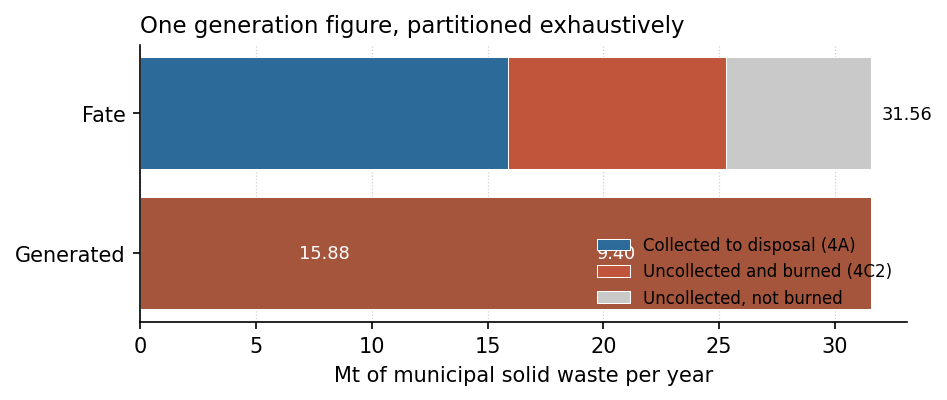
\includegraphics[width=\linewidth]{waste_partition.png}
\caption{The partition. \SI{31.56}{\mega\tonne} of municipal solid waste is generated;
\SI{15.88}{\mega\tonne} is collected and enters the decay model as 4A;
\SI{15.67}{\mega\tonne} is uncollected, of which \SI{9.40}{\mega\tonne} burns as 4C2 and the
remainder is dumped without combustion. The two lower bars sum to the upper one exactly,
which is the property the code asserts rather than checks.}
\label{fig:partition}
\end{figure}

\begin{figure}[htbp]
\centering
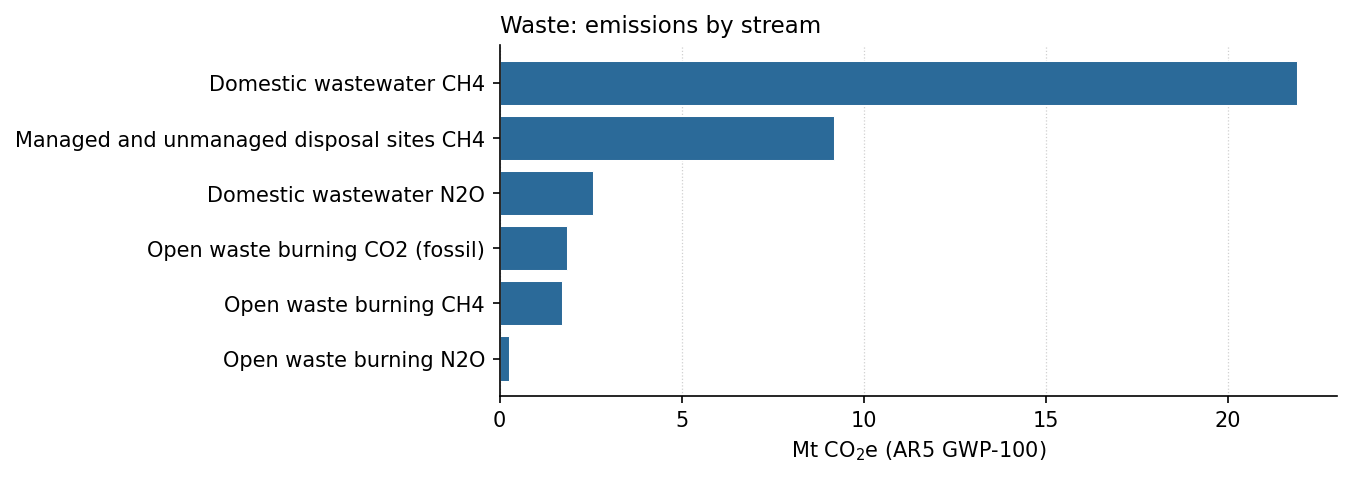
\includegraphics[width=\linewidth]{waste_streams.png}
\caption{Emissions by stream. Domestic wastewater methane alone, at
\SI{21.89}{\mega\tonne} \COe{}, is larger than the other five streams combined.}
\label{fig:streams}
\end{figure}

Methane is \SI{87}{\percent} of the sector, which is why the AR5-to-AR6 difference of
\SI{1.08}{\mega\tonne} is almost entirely a methane effect and why this sector is unusually
sensitive to the metric chosen.

\subsection{Where the uncertainty is}

The factor and activity uncertainties differ substantially by pathway. The current common ensemble reruns the native waste calculation for each realisation and preserves both the waste-fate identity and the asymmetric effluent-N$_2$O factor distribution. Its reference-year conditional interval is \SIrange{25.4}{61.5}{\mega\tonne} CO$_2$e on AR5. This is a parameter interval within the selected management interpretation and source coverage; structural cases remain separate. The standalone sector ensemble and Approach~1 screen retain their own stated settings and are not substituted for the common release interval (Supplementary Note~S1).

\subsection{Sensitivities, published rather than chosen}

\begin{table}[htbp]
\centering
\footnotesize
\begin{tabular}{@{}lrr@{}}
\toprule
\textbf{Assumption} & \textbf{Category (Mt)} & \textbf{Sector (Mt)} \\
\midrule
Sewer MCF \num{0.5} (reported)      & 24.46 & 37.45 \\
Sewer MCF \num{0.1} (river reading) & 15.39 & 28.38 \\
BOD at India's \SI{34}{} g/cap/day  & 21.17 & 34.17 \\
\midrule
Disposal with spin-up (reported)    &  9.17 & 37.45 \\
Disposal without spin-up            &  8.07 & 36.35 \\
\bottomrule
\end{tabular}
\caption{The three assumptions this sector cannot settle, each reported as an alternative
rather than absorbed into the central estimate. Nitrous oxide is invariant under both
wastewater cases because it derives from protein rather than from BOD or sewer condition, so
all rows are category totals including it---a distinction this sector's own output file
previously got wrong.}
\label{tab:sensitivity}
\end{table}

\begin{figure}[htbp]
\centering
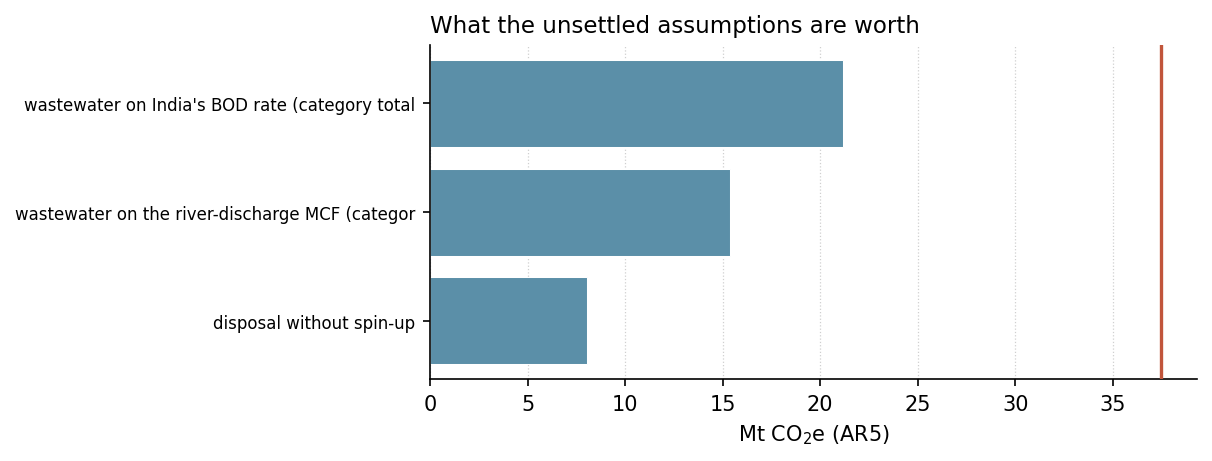
\includegraphics[width=\linewidth]{waste_sensitivity.png}
\caption{The same result as a range around the reported figure. A reader who has to
reconstruct a range from prose will not reconstruct it.}
\label{fig:sensitivity}
\end{figure}

The spin-up row answers a question most first-order-decay implementations answer implicitly:
pre-2000 deposits contribute \SI{12}{\percent} of today's landfill methane. An implementation
that starts at its activity panel is not making no assumption; it is asserting that the
country landfilled nothing before its data begin.

Named structural cases retain their own sewer and management assumptions. They are not
combined into a probability mixture. Conditional parameter intervals describe a specified
case; differences between cases remain a separate sensitivity, including the alternative
partition based on the HIES household route shares in Section~\ref{sec:validation}.

\subsection{Provincial allocation}

\begin{figure}[htbp]
\centering
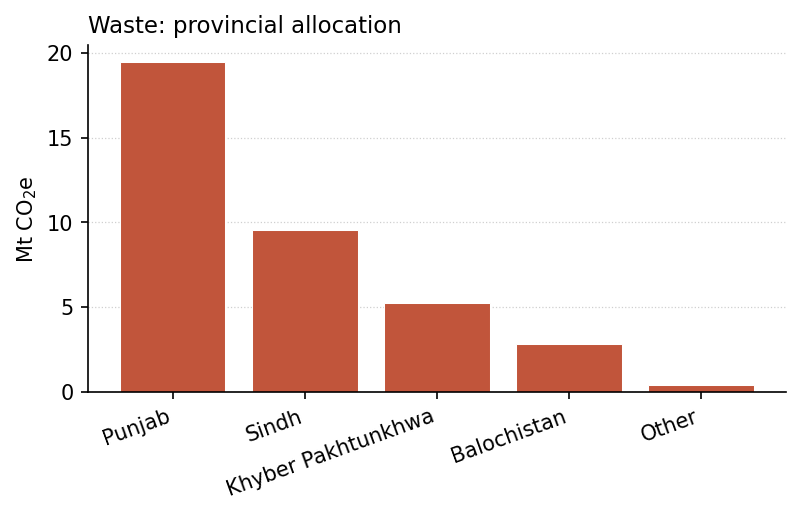
\includegraphics[width=\linewidth]{waste_provincial.png}
\caption{Punjab \SI{19.49}{\mega\tonne}, Sindh \SI{9.55}{\mega\tonne}, Khyber Pakhtunkhwa
\SI{5.21}{\mega\tonne}, Balochistan \SI{2.80}{\mega\tonne} and \SI{0.40}{\mega\tonne} in the
territories. Allocated on the same district population panel that drives generation. This is an
\emph{origin} allocation: population locates where waste and wastewater are produced, and
the split reconciles exactly against each category's national figure---but it carries the
further assumption that release is co-located with origin, which is the stronger claim.}
\label{fig:provincial}
\end{figure}

The provincial pattern follows population closely, which is expected for a sector whose
activity datum \emph{is} population, and is the reason this sector's geography is less
informative than, say, the power sector's. What the allocation locates is the \emph{origin}
of the waste and wastewater---where the generating people live---not the release: disposal
methane is emitted at landfills and dumps, wastewater methane along drains, at treatment
works and at discharge points, and burning at burn sites. What the inventory holds toward
that release geography is a prospective seed only: \num{56} OpenStreetMap
\texttt{landuse=landfill} polygons \citep{osm2026} (ODbL~1.0 derivative database,
\texttt{data/gis/landfills/}), \num{13} of them named, quality-flagged, and touched by no
estimated stream---far too sparse for an SWDS allocation, and registered so the release
can cite what it holds rather than claiming it holds nothing. The three
objects are published SEPARATELY, as the review asked: origin
(\texttt{waste\_district\_2024.csv}), fate (the ledger), and release---the polygons
republished as candidates
(\texttt{outputs/waste\_release\_candidates\_2024.csv}) with an assignment product
(\texttt{outputs/waste\_\allowbreak release\_\allowbreak assignment\_\allowbreak 2024.csv})
whose defining column is EXPLICIT UNASSIGNED MASS: a district's disposal emissions
are assigned only to its own mapped candidates (equal split, capacity unknown and
declared), nothing crosses a district boundary, and \SI{75}{\percent} of the
disposal category stays unassigned across \num{113} districts---the honest measure
of how far a release map is from existing. At provincial resolution
the origin/release distinction is modest, because waste
rarely crosses a provincial boundary between generation and fate; at any finer resolution
the population surface would place landfill methane in residential neighbourhoods, which
is why the sector's ALLOCATION remains origin-based and the limitations
section carries the gap.

\subsection{Contribution to the national inventory}

The category composition separates wastewater methane and N$_2$O, disposal-history methane and burning releases. Their uncertainty and user relevance depend on the species: a small contribution to the GHG aggregate does not imply a small primary PM or other pollutant release. The current native ensemble and pollutant-specific driver diagnostics are used to identify parameter sensitivity, without treating the old Approach~1 category screen as an additive variance decomposition of the nonlinear national ensemble.

\FloatBarrier
% ===========================================================================
\section{Air-Pollutant Co-Emissions}
\label{sec:air}
% ===========================================================================

Open municipal-waste burning uses the same wet/dry burned quantity and fate account as the greenhouse-gas calculation. The FY2023--24 reference burned mass is \SI{9.40}{\mega\tonne}; pollutant-specific garbage-burning factors follow \citet{andreae2019}. Masses are reported in native units. Burning locations are not observed nationally, so the population allocation describes waste origin rather than confirmed release sites.

\begin{table}[htbp]
\centering
\footnotesize
\begin{tabular}{@{}lr@{}}
\toprule
\textbf{Pollutant} & \textbf{kt/yr} \\
\midrule
CO                  & 434.45 \\
NMVOC               & 151.40 \\
\PM{}               &  63.85 \\
HCl                 &  18.43 \\
\NOx{} (as NO$_2$)  &  15.14 \\
Black carbon        &   9.22 \\
\NHthree{}          &   5.92 \\
\SOtwo{}            &   3.29 \\
\bottomrule
\end{tabular}
\caption{Air pollutants from open waste burning, FY2023--24. Mass only; these never enter a
greenhouse-gas total. Computed from the same burned tonnage as the 4C2 emissions above, so the
two describe the same fire. \NOx{} is reported as NO$_2$-equivalent
(Andreae publishes the garbage-burning factor as NO; the conversion is documented on the
factor row), the inventory-wide basis.}
\label{tab:air}
\end{table}

\begin{figure}[htbp]
\centering
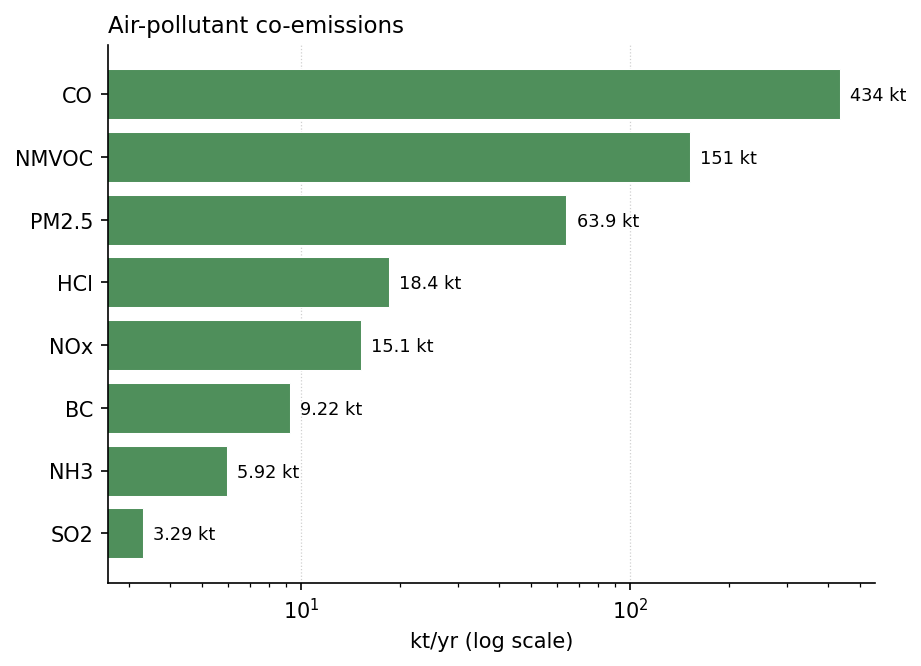
\includegraphics[width=\linewidth]{waste_air.png}
\caption{The same figures on a log axis, which the range demands: carbon monoxide and
sulphur dioxide differ by more than two orders of magnitude, and a linear axis renders
everything below \PM{} as a line of zero width.}
\label{fig:air}
\end{figure}

\subsection{Interpretation of primary particulate releases}

The reference estimate is \SI{63.85}{\kilo\tonne} of primary PM$_{2.5}$. Its relative contribution depends on the compared pollutant, source coverage and household or industrial configuration. No inverse relationship between GHG and pollutant rankings is assumed. Emitted mass does not establish exposure: disposal and burning locations, release conditions, atmospheric transport and chemistry remain outside this calculation.

The common activity account prevents disposal and burning from claiming the same generated waste twice. It does not establish where the uncollected material burns or validate the pollutant factors. The unburned uncollected fraction remains an unresolved fate, rather than an invented combustion destination.

\subsection{Black carbon and hydrogen chloride}

Two entries deserve comment because they are specific to waste rather than generic to
combustion.

Black carbon at \SI{9.22}{\kilo\tonne} is a strong short-lived warming agent that this
inventory reports as mass and does not convert to \COe{}, following the convention that its
metrics remain contested. It is reported because omitting it would understate the climate
relevance of open burning even while the greenhouse-gas total for 4C2 is small.

Hydrogen chloride at \SI{18.43}{\kilo\tonne} appears in no other sector of this inventory and
is a direct consequence of burning chlorinated plastics in the open. It does not quantify dioxin or furan releases, which require separate source-specific methods.

\subsection{Limitations of this layer}

The conditional air ensemble reuses the same bounded waste-fate realisations as the GHG calculation, then applies pollutant-factor uncertainty. Burning-fraction alternatives remain separate structural cases; their endpoints are not confidence limits. The composition is regional rather than Pakistani, which matters more for
pollutants than for greenhouse gases because plastics and textiles drive the chlorine and much
of the particulate. And the factors describe open burning generically rather than the specific
conditions of Pakistani street-side burning---smouldering, damp, and often mixed with organic
waste---whose consequences for incomplete-combustion products require local evidence.

\FloatBarrier
% ===========================================================================
\section{Discussion}
\label{sec:discussion}
% ===========================================================================

\subsection{The methane correction factor, and why it is not resolved here}

The sewer methane correction factor is the largest single assumption in this sector and the
one the evidence does not settle. It deserves the space because how it is handled is a
methodological position, not a parameter choice.

IPCC gives \num{0.5} for stagnant open sewers and \num{0.1} for wastewater discharged to a
flowing, well-aerated body. The distinction was drawn for systems that are clearly one or the
other. Pakistani urban drainage is not: the drains are open, warm, slow-moving and heavily
organically loaded, which is the description \num{0.5} exists for, while a substantial
fraction ultimately discharges to rivers and irrigation channels, which is the description
\num{0.1} exists for. Both descriptions are accurate about different parts of the same system,
and no Pakistani source reports the hydraulic condition of the sewered fraction, which is the
quantity the factor is actually asking about.

The consequence is a factor of \num{1.59} on the sector's largest category:
\SI{24.46}{\mega\tonne} against \SI{15.39}{\mega\tonne}, or \SI{37.45}{\mega\tonne} against
\SI{28.38}{\mega\tonne} for the sector.

\subsubsection{Why external agreement is not a tiebreak}

At \num{0.1} this sector lands close to EDGAR, and it would be easy to present that as
corroboration. It is not, and treating it as one would be a methodological error worth naming
because it is a tempting one.

EDGAR is a model. Its Pakistani wastewater figure rests on its own assumption about the same
unmeasured quantity---the anaerobic fraction of Pakistani sewage---made from the same absence
of Pakistani measurement. If this inventory adopted \num{0.1} because it produces agreement,
the two would agree because both had chosen the same default, and the agreement would then be
cited as though it were evidence about Pakistani drains. That is how a shared assumption
becomes an apparent consensus.

We therefore report \num{0.5} as central, because the physical description of the drains is
the stronger evidence and is specific to Pakistan, and publish \num{0.1} beside it so a user
who weighs the comparator differently can take it. What we do not do is let the comparison
choose.

\subsubsection{What would settle it}

Dissolved-methane concentration and flux measurement on urban drains in two or three Pakistani
cities, sampled across a seasonal cycle to capture the dry-season stagnation and the monsoon
flushing that the two IPCC categories describe separately.

The case for doing it is quantitative rather than rhetorical. Domestic wastewater is
\SI{5.5}{\percent} of Pakistan's national emissions and \SI{13.0}{\percent} of national
inventory variance under Approach~1---the second largest variance contributor of any category
in the country on that screen.
A measurement campaign of a few tens of thousands of dollars would reduce national inventory
uncertainty more than any comparable expenditure elsewhere in the waste or energy sectors.

\subsection{What the closed mass balance buys, and what it does not}

The balance guarantees that the collected and uncollected streams together account for
exactly the waste the country generates, with the burned quantity a declared fraction of the
uncollected stream and the unburned \SI{6.27}{\mega\tonne} carried as an explicit unresolved
fate rather than assigned to either category. That removes a specific class of error---the two
categories drifting into mutual inconsistency as one is updated---and makes the collection rate
an explicit, single, arguable number rather than an implicit consequence of two independent
estimates.

It is worth being precise about what it does not buy, because a closed balance invites
overconfidence. It says nothing about whether the split point is right. The collection rate of
\SI{50.3}{\percent} carries real uncertainty, and moving it moves waste between two fates with
quite different methane yields per tonne: a tonne landfilled decays slowly and anaerobically
over decades, while a tonne burned emits immediately and mostly as \COtwo{}. Nor does it
validate the generation figure itself; a partition of a wrong total still closes.

What it changes is the shape of the argument. A reader who disagrees with the collection rate
can see exactly which two categories move and in which directions, rather than having to work
out whether two independently sourced numbers are mutually consistent.

\subsection{Implications}

Three follow, in descending order of confidence.

\textbf{Wastewater is the sector, and the sector is a measurement problem.} Two-thirds of the
emissions and nearly all of the tractable uncertainty sit in one category whose central
parameter has never been measured in Pakistan. Effort spent refining the solid-waste decay
parameters or the burning composition would improve smaller numbers that are already better
constrained.

\textbf{Open burning matters for air quality, not for climate.} At \SI{0.86}{\percent} of
national \COe{} and roughly \SI{14}{\percent} of national primary \PM{}, it is a category whose case for
intervention rests on exposure. An abatement programme justified on greenhouse-gas grounds
would be hard to defend; the same programme justified on particulate would be
straightforward.

\textbf{The collection rate is a policy variable, not just a parameter.} Because the partition
makes it the single number governing what fraction of waste burns rather than decays,
improving collection is visible in this inventory as a movement between categories. That is
the right structure for evaluating a municipal collection programme, and it is not available
in an inventory whose two categories are estimated independently.

% ===========================================================================
\section{Limitations}
\label{sec:limitations}
% ===========================================================================

\textbf{The sewer methane correction factor is unresolved, and it is the sector.} A factor of
\num{1.59} on two-thirds of the emissions, argued in Section~\ref{sec:discussion}. Both
readings are published; neither is measured.

\textbf{Industrial solid waste and industrial wastewater are not estimated at all.} No national
quantity for either has been compiled here. The categories reported here are municipal and
domestic only, and both gaps carry the notation key NE with that justification, in the
complete sector-4 matrix of \ref{app:completeness}---which also declares biological
treatment (4B) and incineration (4C1) as NE rather than leaving them silently absent.
Industrial wastewater is the more consequential omission: given that domestic wastewater
alone is \SI{5.5}{\percent} of the national inventory, an industrial stream from a textile
and tanning sector of Pakistan's size is unlikely to be negligible.

\textbf{Generation rates are single national values.} The urban and rural per-capita rates do
not vary by province or city size, which is a real simplification for a country whose largest
city and smallest districts differ substantially in consumption and in what they discard. The
rates are regional literature values rather than Pakistani measurements.

\textbf{The collection rate is the softest number in the partition.} The mass balance
closes by construction, but \SI{50.3}{\percent} is an assumption, and it governs how much
waste decays slowly in a landfill versus burns immediately in the street. It is a single
national figure applied through an urban/rural split, when collection in practice varies
between municipalities far more than between those two categories. The one Pakistani survey
that asks the question directly, HIES 2024--25, reports materially less collection than the
assumption (Section~\ref{sec:validation}); its household-route shares are priced as a
structural scenario rather than adopted, because route shares are not mass shares.

\textbf{The burned fraction is a literature value.} That \SI{60}{\percent} of uncollected
waste burns is the least evidenced parameter in the sector and has no Pakistani measurement
behind it at all. It scales open burning linearly, and with it the entire air-pollutant layer
in Section~\ref{sec:air}. Its complement is the fate ledger's unresolved row:
\SI{6.27}{\mega\tonne} of uncollected, unburned waste---dumped to land and
waterways---to which no emissions pathway is applied at all. That choice is now bounded
rather than silent: the scenario table prices the unresolved mass as unmanaged shallow
disposal (sector total \SI{39.87}{\mega\tonne}) and unmanaged deep disposal
(\SI{42.28}{\mega\tonne}) against the reference reading (\SI{37.45}{\mega\tonne}),
on the declared assumption that the dumped stream shares the collected stream's deposit
history and composition. Waterway decay lies between inert and shallow. No probability
attaches to any point in the bound---a disposal-site census, not a better default, is
what would close it.

\textbf{Waste composition is regional, not Pakistani.} The fossil carbon fraction governs how
much of the burning \COtwo{} is reportable, and the plastics and textiles content governs the
chlorine and much of the particulate. A Pakistani waste-characterisation survey would replace
both.

\textbf{No methane recovery is credited and no landfill oxidation applied.} Both are set to
zero because neither is documented at national scale, and both choices bias the disposal
category high if any large Pakistani site does in fact manage its gas or maintain a cover. The
direction of that bias is stated rather than hedged.

\textbf{The spin-up back-projection is an assumption, not data.} Extending the deposit series
to 1960 at \SI{40}{\percent} of the panel's first year is a judgement about Pakistan's waste
history. Its effect is reported---\SI{12}{\percent} of current landfill methane---so a reader
can remove it, but the shape of the back-projection is not evidenced.

\textbf{Uncertainties are large, and honestly so---and honestly asymmetric.}
Five of the six streams carry between
\SI{74}{\percent} and \SI{124}{\percent}; wastewater N$_2$O carries the bounded 150-fold
factor range, and the sector reads $\pm\SI{51.1}{\percent}$ by quadrature with a
parameter-rerun 95\% interval of \SIrange{25.7}{61.4}{\mega\tonne}
(Supplementary Note~S1).
These follow IPCC's own Tier~1 guidance for waste parameters and reflect that the underlying
activity is modelled from population rather than measured at facilities. They are not an
artefact of conservative parameter choice; they are what Tier~1 can say about a country with
no facility-level waste data.

\textbf{Dioxins and furans are not estimated.} Open burning of chlorinated plastics produces
them, and the hydrogen chloride reported in Section~\ref{sec:air} is a marker for the
conditions that do. Estimating them needs a dedicated study rather than a factor applied to
the same tonnage.

% ===========================================================================
\section{Conclusion}
\label{sec:conclusion}
% ===========================================================================

Pakistan's waste sector emitted \SI{37.45}{\mega\tonne} \COe{} in FY2023--24 on AR5 metrics:
\SI{24.46}{\mega\tonne} from domestic wastewater, \SI{9.17}{\mega\tonne} from solid-waste
disposal and \SI{3.83}{\mega\tonne} from open burning. The sector is \SI{8.4}{\percent} of a
ten-sector national inventory and \SI{87}{\percent} methane, which makes it unusually
sensitive to the metric chosen and unusually relevant to near-term mitigation.

Two things generalise beyond this country.

\textbf{An activity figure shared between categories should be partitioned, not estimated
twice.} Solid-waste disposal and open burning describe two fates of one waste stream, and
computing them from one generation figure with $D + U = G$ asserted removes a class of
inconsistency that independent estimation cannot detect. The cost is nil and the gain is that
an argument about the collection rate becomes an argument about where emissions sit rather
than about how much waste exists. The same shape recurs wherever two categories divide one
national quantity.

\textbf{Where an assumption spans a factor approaching two and the evidence does not choose,
the defensible output is both numbers.} The sewer methane correction factor moves this sector
from \SI{37.45}{\mega\tonne} to \SI{28.38}{\mega\tonne}. The lower value happens to agree
better with EDGAR, and adopting it for that reason would have been a mistake: EDGAR is a model
resting on its own assumption about the same unmeasured quantity, so the agreement would have
recorded a shared default as though it were evidence about Pakistani drains. We report
\num{0.5} as central because the physical description of the drains is the stronger and more
specific evidence, publish \num{0.1} alongside, and name what would settle it.

Domestic wastewater remains a consequential uncertainty because sewer fate and discharge conditions are not observed comprehensively. Seasonal dissolved-methane and flux evidence could distinguish the retained structural cases. Open-burning pollutant factors and burn locations require separate evidence; a population-based waste-origin allocation is not an exposure estimate. The extended release advances the existing history rather than inventing annual management observations.

\FloatBarrier

% ---------------------------------------------------------------------------
\section*{Code and data availability}
% ---------------------------------------------------------------------------

The calculation engine, the activity data, the parameter tables and every output quoted here
are version-controlled in the inventory repository
(\url{https://github.com/PakAirQuality/pakistan-emissions-sectors}) and reproduce from a single command. The sector is regenerated with
\texttt{python3 -m pkinv.sectors.waste.run\_waste}; \ref{app:repro} gives the full
sequence. Every number printed in this paper is read from a generated CSV rather than
transcribed, and a test asserts that the manuscript and the engine agree.

% ---------------------------------------------------------------------------
\bibliographystyle{elsarticle-harv}
\bibliography{../../paper_common/references}

% ---------------------------------------------------------------------------
\appendix
\renewcommand{\thetable}{\arabic{table}}%
\renewcommand{\thefigure}{\arabic{figure}}%
% ===========================================================================
\section{Reproduction}
\label{app:repro}
% ===========================================================================

The sector runs on Python 3.11 with no compiled dependencies:

\begin{verbatim}
pip install -e .
python3 -m pkinv.sectors.waste.run_waste
python3 -m pkinv.sectors.waste.air_pollutants
python3 -m pkinv.sectors.waste.uncertainty
\end{verbatim}

which writes \texttt{waste\_totals\_2024.csv}, \texttt{waste\_by\_stream\_2024.csv},
\texttt{waste\_provincial\_2024.csv}, \texttt{waste\_air\_pollutants\_2024.csv},
\texttt{waste\_ledger\_2024.csv}, the twelve-month layer
(\texttt{waste\_\allowbreak monthly\_\allowbreak 2024.csv}, each month's share with the emissions it implies and
the basis of the shape), the three uncertainty files (\texttt{waste\_\allowbreak uncertainty\_\allowbreak 2024.csv},
\texttt{waste\_\allowbreak uncertainty\_\allowbreak inputs\_\allowbreak 2024.csv} and
\texttt{waste\_\allowbreak uncertainty\_\allowbreak scenarios\_\allowbreak 2024.csv}) and
\texttt{waste\_report.md} to \texttt{outputs/}. The generated appendix tables are rendered
by the three \texttt{scripts/make\_waste\_*\_table.py} generators, and a test asserts each
committed table matches a fresh regeneration. The cross-sector layer that places this sector
in the national inventory is:

\begin{verbatim}
python3 -m pkinv.report.national_rollup
python3 -m pkinv.report.key_categories_all
python3 -m pkinv.report.uncertainty_all
\end{verbatim}

Figures are regenerated with \texttt{python3 -m pkinv.report.figures} and copied into this
manuscript by \texttt{python3 scripts/sync\_figures.py}; a test fails if any shipped figure
differs from the output it plots. The full suite, including the sector's own arithmetic tests
and the checks that every number printed above matches its source CSV, runs with
\texttt{python3 -m unittest discover tests}.

% ===========================================================================
\section{Sources}
\label{app:sources}
% ===========================================================================

Population is the 2023 Population and Housing Census \citep{pbscensus2023}, interpolated to a
district panel. Waste generation rates and composition derive from the Pak-EPA eight-city
survey \citep{pakepa1996}, which \citet{kaza2018} re-bins; collection coverage is the Pakistan
row of \citet{kaza2018}. Sanitation shares are the WHO/UNICEF Joint Monitoring Programme's
Pakistani series \citep{jmp2023}. Emission factors and model parameters are IPCC 2006
Guidelines Volume~5 defaults \citep{ipcc2006waste}, with the wastewater nitrous oxide method
and its factors from the 2019 Refinement \citep{ipcc2019}; air-pollutant factors are the
\citet{andreae2019} garbage-burning assessment. External comparisons are EDGAR's year-matched
series \citep{edgar2025booklet} and Climate TRACE \citep{climatetrace}.

Every factor in the repository cites its source table, and a provenance test asserts that none
lacks a citation and that any informally sourced value is explicitly declared as such.

% ===========================================================================
\section{Supplementary Note: the two sensitivity conventions}
\label{app:sens}
% ===========================================================================

Both wastewater sensitivities move methane only. Nitrous oxide in 4D1 is computed from protein
consumption rather than from BOD, so it is invariant under a change to either the sewer
correction factor or the BOD rate.

This is worth an appendix because getting it wrong is easy and was in fact got wrong here. The
sector's output file originally wrote the two sensitivity rows as \emph{methane only} into a
column whose every other row was a category total. A reader comparing the reported
\SI{24.46}{\mega\tonne} against the river-discharge row's \SI{12.82}{\mega\tonne} would have
computed a lever of \num{1.91} where the real one is \num{1.59}, and the file disagreed with
the module's own printed summary, which had always added the nitrous oxide back.

The rows now carry category totals and are labelled as such. The general point is that a
sensitivity is only interpretable against a stated basis, and a sensitivity table mixing bases
within one column is worse than no sensitivity table, because it invites a subtraction that
looks valid.

% ===========================================================================
\section{Supplementary Note S1: Uncertainty, Approach 1 against Approach 2}
\label{app:uncertainty}
% ===========================================================================

This note carries the sector's uncertainty treatment. An earlier edition's form was
indefensible and was rebuilt: the effluent N$_2$O factor carried a symmetric
$\pm\SI{100}{\percent}$ against its own published 500-fold range (0.0005--0.25, the 2006
Guidelines'), three wastewater parameters carried zero uncertainty against stated ranges,
and the Monte Carlo
drew component totals that could not promise the fate ledger's closure in any single
realisation. All three defects are repaired here, and every published band on this page
moved as a consequence---which is the repair working, not a revision of the inventory
(the repair left the deterministic totals unchanged to the last digit).

The bands moved a second time when the nitrous oxide estimate went onto the method of the
2019 Refinement (Section~\ref{sec:methods}), and that move is a revision of the inventory:
wastewater N$_2$O fell from \SI{11.45}{} to \SI{9.71}{\giga\gram} and the sector from
\SI{37.91}{} to \SI{37.45}{\mega\tonne}. The Refinement prints the effluent factor's range
as 0.0005--0.075, a 150-fold range, and that is the range drawn below; the 2006 equation,
drawn over its own range, is kept as the alternative.

\subsection{The headline interval: a parameter-rerun Monte Carlo, ledger-true by
construction}

The sector's published interval now comes from a Monte Carlo that draws the sector's
\emph{inputs}---generation rates, the collection partition, composition, decay and
correction factors---and reruns the full engine for every one of \num{10000} realisations,
asserting the fate identities $D+U=G$ and $B+R=U$ inside each draw before it is accepted
(\texttt{outputs/waste\_parameter\_mc\_2024.csv}). Covariance is not modelled; it
\emph{emerges}: the shared generation figure moves disposal and burning together, the
uncollected fraction moves mass between them with opposite signs, and the decay rate's
nonlinearity through the deposit stock is exact rather than linearised.

The effluent N$_2$O factor is drawn from a bounded split-triangular in log space over its
published range, with the IPCC default \num{0.005} as mode and median: the endpoints bound
every draw, half the probability lies each side of the default, and the density falls to
zero at the published limits. Its 95\% interval runs from about one sixth of the default
to \num{8.2} times it---a \num{49}-fold span, wide because the evidence is
wide---against the \num{6.6}-fold span the old symmetric declaration smuggled in.

\begin{table*}[htbp]
\centering
\footnotesize
\begin{tabular}{@{}lrrrrr@{}}
\toprule
\textbf{Category} & \textbf{Det.} & \textbf{Mean} & \textbf{P2.5} & \textbf{P50} &
\textbf{P97.5} \\
\midrule
Domestic wastewater  & 24.46 & 26.53 & 14.88 & 25.07 & 47.19 \\
Solid-waste disposal &  9.17 &  9.21 &  3.61 &  8.73 & 17.58 \\
Open burning         &  3.83 &  3.82 &  1.65 &  3.54 &  7.54 \\
\midrule
\textbf{Sector} & \textbf{37.45} & \textbf{39.55} & \textbf{25.70} & \textbf{38.30} &
\textbf{61.42} \\
\bottomrule
\end{tabular}
\caption{The parameter-rerun Monte Carlo, Mt \COe{} (AR5): \num{10000} input draws on
the published seed \num{4421} (the \texttt{seed} column of
\texttt{outputs/waste\_parameter\_mc\_2024.csv}), the
sector rebuilt and the fate ledger asserted in every realisation. The interval is
deliberately asymmetric---the mean sits above the deterministic value and the upper arm is
longer than the lower---because the effluent factor's published range is asymmetric
and is now priced rather than symmetrised. No symmetric $\pm$ percentage can represent
this shape, which is why the quadrature figures below are reported as cross-checks rather
than as the sector interval.}
\label{tab:rerunmc}
\end{table*}

\subsection{The quadrature cross-checks, re-anchored}

Under IPCC Approach~1---each component's relative uncertainty combined in
quadrature---the sector reads $\pm\SI{51.1}{\percent}$, against \SI{47.8}{} before the
repair; Approach~1 consumes the effluent factor's bounded shape as its log-variance-matched symmetric equivalent (about \SI{267}{\percent}), the honest degradation for a surface carrying one number. An earlier national engine re-expressed this sector as
component-lognormals at the width then declared, and its upper arm arrived nationally at
\SI{63.5}{\mega\tonne}, well below the rerun engine's on the 2006 range then drawn---a
material compression of the upper tail. \textbf{The national engine consumes this sector's own
rerun draws} (a persisted \num{100000}-draw file on seed \num{4421}, whose first
\num{10000} draws are bit-identical to the rerun table above; hash in the release
manifest), so the national rows below ARE the sector engine's quantiles.

\begin{table}[htbp]
\centering
\footnotesize
\begin{tabular}{@{}lrrrr@{}}
\toprule
\textbf{Category} & \textbf{Mean} & \textbf{P2.5} & \textbf{P97.5} & \textbf{$\pm$\%} \\
\midrule
Domestic wastewater  & 26.51 & 14.77 & 46.57 & 63.4 \\
Solid-waste disposal &  9.15 &  3.61 & 17.50 & 80.2 \\
Open burning         &  3.83 &  1.65 &  7.70 & 85.7 \\
\midrule
\textbf{Sector}      & \textbf{39.48} & \textbf{25.47} & \textbf{60.93} & \textbf{46.4} \\
\bottomrule
\end{tabular}
\caption{This sector's rows in the NATIONAL Monte Carlo: the sector's own
parameter-rerun draws, injected as a \num{100000}-realisation superset of the
\num{10000}-draw table above (seed \num{4421}; the small quantile differences against
that table are draw count, bounded by the published convergence diagnostics). Mt \COe{}
(AR5). The $\pm$\% column is the symmetric summary; the published CSV carries the
asymmetric $-$/$+$ arms.}
\label{tab:mc}
\end{table}

\subsection{Why the treatments differ, and what the difference says}

The quadrature figure ($\pm\SI{51.1}{\percent}$) is the analytic limit of a symmetric,
independent, moderate-uncertainty simulation---and the rerun engine is deliberately none
of those, so its $\pm\SI{46.4}{\percent}$ symmetric summary (really
$-\SI{33.3}{\percent}/+\SI{59.5}{\percent}$ about the median) stands apart, and the
divergence is the information.

Within categories the right-skew is now carried, not hidden: solid-waste disposal is
$\pm\SI{79.8}{\percent}$ analytically and $\pm\SI{80.2}{\percent}$ in the injected
simulation, its simulated median of \SI{8.66}{\mega\tonne} below its mean of
\SI{9.15}{\mega\tonne}---a long right tail no symmetric half-width can represent. A reader
taking $\SI{9.15}{} \pm \SI{79.8}{\percent}$ as symmetric would infer a lower bound near
\SI{1.8}{\mega\tonne}; the simulation puts the 2.5th percentile at \SI{3.61}{\mega\tonne}
and the 97.5th at \SI{17.50}{\mega\tonne}. The true interval is narrower below and wider
above---and for wastewater, whose factor evidence covers a hundred-and-fifty-fold published range, the
bounded rerun treatment now states how much wider ALL THE WAY TO THE NATIONAL ROW
($+\SI{85.8}{\percent}$ upper arm on the wastewater category).

\subsection{The sector is unaffected by fossil-factor correlation}

The national inventory this sector belongs to reports a second Monte-Carlo scenario in which
the shared IPCC fuel-carbon factors are drawn as one correlated realisation across every
fuel-burning sector, on the reasoning that there is one carbon content of the diesel a country
burns and if the default is wrong it is wrong everywhere at once.

Waste barely moves: $\pm\SI{46.4}{\percent}$ independent against $\pm\SI{46.4}{\percent}$
correlated. That is the expected result and worth stating as an internal check rather than a
finding. Only the \COtwo{} from open burning derives from a fossil-carbon factor at all, and
it is \SI{4.9}{\percent} of the sector; the methane that dominates comes from decay and
anaerobic digestion, which share no factor with any combustion sector. A sector that moved
materially under that scenario would indicate a factor being shared where it should not be.

\subsection{What dominates, and what a measurement would buy}

Decomposing the sector variance by category under Approach~1 gives domestic wastewater
\SI{13.0}{\percent} of \emph{national} inventory variance, solid-waste disposal
\SI{2.3}{\percent} and open burning \SI{0.2}{\percent}.

Two consequences follow. Effort on open burning cannot improve the national inventory
materially however well it is done---its entire variance contribution is a fifth of one
percent---though it remains the sector's most important category for air quality. And the
wastewater band has TWO named drivers, not one. An
earlier edition of this note claimed the sewer methane correction factor unquestionably
dominated; that claim was an artefact of pricing the effluent N$_2$O factor at a symmetric
$\pm\SI{100}{\percent}$ against the 500-fold range the 2006 Guidelines printed. What the
effluent factor carries is now read from the released ensemble and not from a ranking of
parameters: frozen at its default in a rerun of the waste engine on the ensemble's own
draws, it accounts for \SI{4.1}{\percent} of national variance and \SI{4.8}{\percent} of the
excess in the upper tail, where the wastewater category as a whole accounts for
\SI{9.0}{\percent} and \SI{10.5}{\percent}
(\texttt{outputs/pakemis\_uncertainty\_drivers.csv}). The
sewer factor's structural reading (\num{0.5} against \num{0.1}, a factor of \num{1.59} on
the CH$_4$ side) is a scenario and has no share in that decomposition. What a measurement
would buy therefore splits by pathway: a
dissolved-methane campaign on urban drains resolves the sewer weights, and an
effluent-pathway N$_2$O measurement---which no Pakistani study provides---is what would
collapse the factor range that now sets the sector's ceiling.

That is the quantitative case for the measurement campaign proposed in
Section~\ref{sec:discussion}, and it is a stronger case than the sector's size alone would
make.

\subsection{The partition's couplings, and a grouped Approach 1}

The pooled treatment above draws the six components independently, but two of the three
categories are built from one generation figure and one collection coverage, and those
couplings pull in opposite directions. The generation rates are shared \emph{positively}: if
Pakistanis generate more waste than the Pak-EPA rates say, disposal and burning are both
underestimated at once. The uncollected fractions are shared \emph{negatively}: a tonne not
collected is a tonne unavailable to the decay model and available to burn, so the partition
term partially cancels between 4A and 4C2. A grouped Approach~1 carrying both couplings
analytically---shared terms linear with their signed elasticities, residuals in
quadrature---gives $\pm\SI{51.6}{\percent}$ against the independent
$\pm\SI{51.1}{\percent}$ (\texttt{outputs/waste\_uncertainty\_2024.csv}). The generation
coupling outweighs the anticorrelation, so the pooled treatment slightly \emph{understates}
the sector band; the two effects are decomposed on the output row rather than netted
silently.

\subsection{Structural scenarios: the sewer as a mixture, the partition under survey
evidence}

The IPCC choice this sector cannot settle---stagnant-sewer \num{0.5} against
river-discharge \num{0.1}---is physically a statement about \emph{weights}: Pakistani
drains stagnate in the dry season and flush in the monsoon, so the real system is a mixture
of regimes, not a single row of Table~6.3. Because the methane equation is linear in the
correction factor, any mixture is exactly a scalar, and the configurations below are named
structural scenarios with conditional intervals rather than a probability distribution over
weights the country has never measured. Each row reruns the full sector
(\texttt{outputs/waste\_uncertainty\_scenarios\_2024.csv}; \num{10000} draws on seed
\num{4321}---its own stream, so the pooled national stream's seed \num{42} is
untouched; an earlier edition called this seed ``private'', which conflated
stream separation with non-publication and made the scenario intervals
irreproducible from the manuscript).

\begin{table}[htbp]
\centering
\footnotesize
\begin{tabular}{@{}lrrr@{}}
\toprule
\textbf{Scenario} & \textbf{Mt} & \textbf{P2.5} & \textbf{P97.5} \\
\midrule
Reference (sewer \num{0.5})            & 37.45 & 22.58 & 60.71 \\
All-stagnant mixture endpoint          & 37.45 & 22.45 & 60.26 \\
All-flowing mixture endpoint           & 28.38 & 17.54 & 44.92 \\
River MCF at its floor (\num{0})       & 26.12 & 16.41 & 41.22 \\
River MCF at its ceiling (\num{0.2})   & 30.65 & 18.93 & 48.48 \\
Equal stagnant/flowing mix             & 32.92 & 20.04 & 52.04 \\
BOD at India's rate                    & 34.17 & 20.84 & 54.60 \\
Disposal without spin-up               & 36.35 & 21.75 & 58.61 \\
HIES household route shares            & 35.56 & 21.78 & 57.72 \\
Unresolved fate: inert (reference)     & 37.45 & 22.38 & 59.61 \\
Unresolved fate: shallow dumps         & 39.87 & 24.19 & 64.13 \\
Unresolved fate: deep dumps            & 42.28 & 25.61 & 66.91 \\
Effluent EF at its floor (\num{0.0005}) & 35.17 & \multicolumn{2}{c}{endpoint, no interval} \\
Effluent EF at its ceiling (\num{0.075}) & 73.03 & \multicolumn{2}{c}{endpoint, no interval} \\
\bottomrule
\end{tabular}
\caption{Structural scenarios, sector totals, AR5. Deterministic value with the 95\%
interval of a conditional Monte Carlo (\num{10000} draws, seed \num{4321}): each interval is
conditional on its configuration, and no probability is assigned across rows. The
all-stagnant endpoint is identical to the reference by construction, which is the proof
that the mixture representation changes nothing; the all-flowing endpoint reproduces the
published river-discharge sensitivity, and the two river-MCF rows price that reading's OWN
published 0--0.2 range, which previously carried a silent zero. The three unresolved-fate
rows are a FORMAL STRUCTURAL FAMILY (\texttt{unresolved\_fate}, named in
their scenario notes): they bound the fate ledger's \SI{6.27}{\mega\tonne} no-pathway
remainder between inert and
unmanaged deep disposal, on the declared deposit-history assumption stated in the scenario
notes. The reference member (inert) is an EVIDENCE-ABSENCE choice, not a physical
claim---no site census says where the dumped mass sits---and the family members may
not be quoted separately. The two effluent-EF rows state the discrete endpoints of the 150-fold published
range the bounded draw prices continuously---at the ceiling, wastewater N$_2$O alone
reaches about \SI{38}{\mega\tonne}; on the 2006 Guidelines' ceiling of \num{0.25} it reached
about \SI{152}{\mega\tonne}, which is the arithmetic an external reader used to
show the old $\pm\SI{100}{\percent}$ was incompatible with the stated evidence. The
endpoints are deliberately published without conditional intervals: an interval around a
deliberately extreme point would manufacture spread the evidence does not license.}
\label{tab:wastescenarios}
\end{table}

Two rows carry the new information. The equal mixture---half the sewered load stagnant,
half flowing, with the treated sliver of \SI{1}{\percent} at the not-well-managed plant
factor---gives an effective correction factor of \num{0.300} and a sector of
\SI{32.92}{\mega\tonne}: the physically plausible seasonal reading sits closer to the
central estimate than to the river reading. And the HIES configuration prices the survey
evidence of Section~\ref{sec:validation}: moving the partition to the household route
shares \emph{lowers} the sector to \SI{35.56}{\mega\tonne}, because the extra uncollected
tonnage burns immediately instead of decaying at the disposal correction factor---the
direction a reader might not guess, and the reason the partition's couplings deserve the
grouped treatment above.

Five further rows of the same file price what the nitrous oxide method declares and does
not measure. The equation of the 2006 Guidelines, the reference before, gives a sector of
\SI{37.91}{\mega\tonne}. Reading the Refinement's Figure~6.1 literally---the nitrogen
leaving septic tanks, latrines, unimproved facilities and open defecation goes to soil, so
that only sewered nitrogen is effluent---gives \SI{35.87}{\mega\tonne}; the reference
follows Equation~6.8, which sums every pathway. The Refinement's factor for
nutrient-impacted or hypoxic receiving waters (\num{0.019}) on every discharge gives
\SI{44.57}{\mega\tonne}, an endpoint without an interval, because no classification of
Pakistan's receiving waters is compiled. Septic tanks with a land dispersal field give
\SI{37.72}{\mega\tonne}, and twice the declared treated share of sewered flow gives
\SI{37.48}{\mega\tonne}. The two methods are also compared on the same draws
(\texttt{outputs/pakemis\_wastewater\_method\_comparison.csv}): the wastewater category's
95\% interval is \SIrange{14.9}{47.2}{\mega\tonne} under the 2019 method and
\SIrange{15.1}{85.2}{\mega\tonne} under the 2006 method drawn over its own range, and the
national interval is \SIrange{399.8}{505.4}{\mega\tonne} against
\SIrange{401.0}{524.4}{\mega\tonne}.

% GENERATED by scripts/make_waste_tier_table.py - do not hand-edit;
% a test asserts this file matches a fresh regeneration, and the generator
% asserts every parameter value it quotes against data/waste_params.csv.
% ===========================================================================
\section{Supplementary Table: tier status by component}
\label{app:tiers}
% ===========================================================================

Tier status differs by component. The three categories share one activity
basis -- the district population panel -- but carry different levels of
country-specific characterisation, and two pieces of the sector are not on
the IPCC tier ladder at all. One word for the whole sector would either
overstate the factors or understate the activity.

\begin{table*}[htbp]
\centering
\scriptsize
\begin{tabular}{@{}llp{0.55\linewidth}@{}}
\toprule
\textbf{Component} & \textbf{Status} & \textbf{Basis} \\
\midrule
4A First Order Decay & Tier 1, country-specific activity & IPCC Vol 5 Ch 3 FOD with default $k$ (0.065), DOC$_f$, $F$ and the uncategorised-site MCF (0.6) over a district census population panel and Pakistani generation rates (0.453 / 0.283 kg/cap/day, Pak-EPA 1996). The activity is country-specific; every decay parameter is a default, and the MCF stands in for a site-type census Pakistan has never published. \\[2pt]
4C2 Open burning & Tier 1, country-specific activity & IPCC Eq 5.7 over the uncollected stream (0.30 urban / 0.70 rural, What a Waste) $\times$ the Box 5.1 burned fraction (0.60), with the Pak-EPA composition supplying carbon and dry matter. The burned fraction has no Pakistani measurement behind it. \\[2pt]
4C2 air-pollutant layer & Field factors (not an IPCC tier) & Andreae 2019 garbage-burning factors on the identical burned mass. The IPCC tier ladder classifies greenhouse-gas estimation; a field-measurement factor set for co-emitted pollutants sits beside it, not on it. \\[2pt]
4D1 CH$_4$ & Tier 1, stratified activity & IPCC Vol 5 Ch 6 defaults (BOD 40 g/cap/day regional, $B_0$ 0.6) over the same population panel stratified by the JMP sanitation split - the stratification is country-specific, the factors are defaults, and the sewer MCF (0.5 central, 0.1 published alongside) is the sector's deciding judgement. \\[2pt]
4D1 N$_2$O & Tier 1 & FAOSTAT protein through the 2019 Refinement's nitrogen chain; the effluent factor's published range spans a factor of 150, the softest number in the sector. \\[2pt]
Provincial allocation & Country-specific allocation (not a tier) & Three distinct district-population-derived proxies (burning, disposal, wastewater load), reconciling exactly to each category's national figure. IPCC tiers classify estimation, not allocation. \\[2pt]
\bottomrule
\end{tabular}
\caption{Tier status by component. Generated; the parameter values quoted
are asserted against \texttt{data/waste\_params.csv} at generation time.}
\label{tab:tierstatus}
\end{table*}

% GENERATED by scripts/make_waste_factor_table.py - do not hand-edit;
% a test asserts this file matches a fresh regeneration of the data files.
% ===========================================================================
\section{Supplementary Table: full factor and parameter provenance}
\label{app:factors}
% ===========================================================================

Every parameter and factor the sector uses, with value, declared 95\%
uncertainty, PRICED BOUNDS where the source publishes a range, and abridged
source, rendered from the versioned data files the engine reads. Note the
deliberate basis differences the compact table in the
body cannot carry: burning CH$_4$ is per WET tonne and N$_2$O per DRY tonne;
the NO$_x$ factor is converted to NO$_2$-equivalent ($\times 46/30$) from
Andreae's published NO; and the two oxidation factors describe two different
physical situations and must not be reconciled
(Section~\ref{sec:factors}). The bounds column exists because a published
range beside a $\pm$\% that could not
carry it is a contradiction: such a parameter is now either drawn from those bounds (the effluent N$_2$O factor,
bounded split-triangular in log space) or priced by named endpoint scenarios
(Section~\ref{app:uncertainty}); a dash means the source states no range.

\begin{table*}[htbp]
\centering
\tiny
\begin{tabular}{@{}lrlrlp{0.40\linewidth}@{}}
\toprule
\textbf{Parameter} & \textbf{Value} & \textbf{Unit} & \textbf{$\pm$\%} & \textbf{Bounds} & \textbf{Source (abridged)} \\
\midrule
gen\_rate\_urban & 0.453 & kg/capita/day & 40 & 0.283--0.613 & Pak-EPA / EPMC 1996 National Study on Privatization of Solid Waste Management in Eight Cities of Pakistan, Table 3 (remaining urb\ldots \\
gen\_rate\_rural & 0.283 & kg/capita/day & 60 & -- & Pak-EPA / EPMC 1996, Table 3 (rural areas) \\
uncollected\_urban & 0.3 & fraction & 30 & -- & World Bank What a Waste 2.0 (Kaza et al. 2018) Pakistan row: urban collection coverage 70\% \\
uncollected\_rural & 0.7 & fraction & 30 & -- & World Bank What a Waste 2.0 (Kaza et al. 2018) Pakistan row: rural collection coverage 30\% \\
burned\_fraction & 0.6 & fraction & 50 & -- & IPCC 2006 GL Vol 5 Ch 5 Box 5.1 \\
oxidation\_factor & 0.71 & fraction & 8 & -- & IPCC 2019 Refinement Vol 5 Ch 5 Table 5.2 (Updated) Note 3; Yamada et al. 2010 \\
oxidation\_factor\_2006 & 0.58 & fraction & 15 & -- & IPCC 2006 GL Vol 5 Ch 5 Table 5.2 Note 3 (US-EPA 1997) \\
dry\_matter & 0.7 & fraction & 20 & -- & Derived: Pak-EPA 1996 composition weighted by IPCC 2006 GL Vol 5 Ch 2 Table 2.4 dry-matter fractions \\
fossil\_c\_per\_wet\_t & 0.0757 & t fossil C per t wet waste & 45 & -- & Derived: Pak-EPA 1996 composition x IPCC 2006 GL Vol 5 Ch 2 Table 2.4 (dm \\
total\_c\_per\_wet\_t & 0.2195 & t C per t wet waste & 35 & -- & Derived: same composition and table with FCF set to 1 \\
swds\_k & 0.065 & 1/yr & 25 & 0.05--0.08 & IPCC 2006 GL Vol 5 Ch 3 Table 3.3, bulk waste, tropical dry (MAT > 20 C, MAP < 1000 mm): default 0.065, range 0.05-0.08 \\
swds\_delay\_months & 6 & months & -- & -- & IPCC 2019 Refinement Vol 5 Ch 3 (reaction delay) \\
swds\_docf & 0.5 & fraction & 20 & -- & IPCC 2006 GL Vol 5 Ch 3 s3.2.3: 'The recommended default value for DOCf is 0.5' \\
swds\_mcf & 0.6 & fraction & 35 & -- & IPCC 2006 GL Vol 5 Ch 3 Table 3.1, 'Uncategorised SWDS' \\
swds\_f & 0.5 & fraction & 10 & -- & IPCC 2006 GL Vol 5 Ch 3 s3.2.3: 'Most waste in SWDS generates a gas with approximately 50 percent CH4 ... use of the IPCC default\ldots \\
swds\_oxidation & 0 & fraction & 0 & -- & IPCC 2006 GL Vol 5 Ch 3 Table 3.2: OX = 0 for managed, unmanaged and uncategorised SWDS \\
swds\_recovery\_t & 0 & tonnes CH4/yr & 0 & -- & No landfill-gas recovery is operating in Pakistan at national scale \\
swds\_backprojection & 40 & percent & -- & -- & Judgement: population before 2000 is back-projected from the panel's own first-decade growth rate \\
ww\_bod\_g\_per\_cap\_day & 40 & g BOD/person/day & 30 & 35--45 & IPCC 2006 GL Vol 5 Ch 6 Table 6.4, 'Asia, Middle East, Latin America' (range 35-45) \\
ww\_bod\_india & 34 & g BOD/person/day & 30 & 27--41 & IPCC 2006 GL Vol 5 Ch 6 Table 6.4, India (range 27-41) \\
ww\_bo & 0.6 & kg CH4/kg BOD & 30 & -- & IPCC 2006 GL Vol 5 Ch 6 Table 6.2, maximum CH4 producing capacity for domestic wastewater \\
ww\_mcf\_sewer & 0.5 & fraction & 60 & 0.4--0.8 & IPCC 2006 GL Vol 5 Ch 6 Table 6.3, 'Stagnant sewer (open and warm)' (range 0.4-0.8) \\
ww\_mcf\_sewer\_river & 0.1 & fraction & 0 & 0--0.2 & IPCC 2006 GL Vol 5 Ch 6 Table 6.3, 'Sea, river and lake discharge' (range 0-0.2) \\
ww\_mcf\_septic & 0.5 & fraction & 0 & -- & IPCC 2006 GL Vol 5 Ch 6 Table 6.3, 'Septic system: half of BOD settles in anaerobic tank' (range given as 0.5, no spread) \\
ww\_mcf\_latrine & 0.1 & fraction & 50 & 0.05--0.15 & IPCC 2006 GL Vol 5 Ch 6 Table 6.3, 'Latrine: dry climate, ground water table lower than latrine, small family (3-5 persons)' (ran\ldots \\
ww\_mcf\_open & 0 & fraction & 0 & -- & IPCC 2006 GL Vol 5 Ch 6 Table 6.3 has no row for open defecation \\
ww\_industrial\_factor & 1.25 & fraction & 20 & -- & IPCC 2006 GL Vol 5 Ch 6 Eq 6.3, correction factor I for additional industrial BOD discharged into sewers (default 1.25 for collec\ldots \\
ww\_f\_npr & 0.16 & kg N/kg protein & 10 & 0.15--0.17 & IPCC 2019 Refinement Vol 5 Ch 6 (data/raw/ipcc/19R\_V5\_6\_Ch06\_Wastewater.pdf), Eq 6.10 and updated Table 6.11 (PDF p. 43): fra\ldots \\
ww\_f\_non\_con & 1.1 & fraction & 10 & 1--1.4 & IPCC 2019 Refinement Vol 5 Ch 6 (data/raw/ipcc/19R\_V5\_6\_Ch06\_Wastewater.pdf), updated Table 6.11 (PDF p. 43): factor for non-\ldots \\
ww\_f\_ind\_com & 1.25 & fraction & 20 & 1--1.5 & IPCC 2019 Refinement Vol 5 Ch 6 (data/raw/ipcc/19R\_V5\_6\_Ch06\_Wastewater.pdf), Eq 6.10 and updated Table 6.11 (PDF pp. 42-43):\ldots \\
ww\_ef\_effluent & 0.005 & kg N2O-N/kg N & bounded split-tri.\ (log) & 0.0005--0.075 & IPCC 2019 Refinement Vol 5 Ch 6 (data/raw/ipcc/19R\_V5\_6\_Ch06\_Wastewater.pdf), new Table 6.8A (PDF p. 39): freshwater, estuari\ldots \\
ww\_mcf\_treated & 0.3 & fraction & 0 & 0.2--0.4 & IPCC 2006 GL Vol 5 Ch 6 Table 6.3, 'Centralised, aerobic treatment plant' - not well managed / overloaded (range 0.2-0.4; well-ma\ldots \\
ww\_treated\_share & 0.01 & fraction & 0 & 0.005--0.02 & Declared scenario weight; no measured national treatment share is compiled here \\
ww\_n\_sludge\_kg & 0 & kg N/yr & -- & -- & IPCC 2006 GL Vol 5 Ch 6 Eq 6.8, N\_SLUDGE: nitrogen removed with sludge, default zero \\
ww\_n2o\_method\_2019 & 1 & switch & -- & -- & This inventory's choice of method for domestic wastewater nitrous oxide \\
ww\_f\_pc & 0.96 & fraction & 5 & -- & IPCC 2019 Refinement Vol 5 Ch 6 (data/raw/ipcc/19R\_V5\_6\_Ch06\_Wastewater.pdf), new Table 6.10A (PDF p. 41): protein consumed a\ldots \\
ww\_n\_hh & 1.1 & fraction & bounded split-tri.\ (log) & 1.07--1.17 & IPCC 2019 Refinement Vol 5 Ch 6 (data/raw/ipcc/19R\_V5\_6\_Ch06\_Wastewater.pdf), Eq 6.10 (PDF p. 40): additional nitrogen from h\ldots \\
ww\_f\_ind\_com\_decentralised & 1 & fraction & 0 & -- & IPCC 2019 Refinement Vol 5 Ch 6 (data/raw/ipcc/19R\_V5\_6\_Ch06\_Wastewater.pdf), text under Table 6.10B (PDF p. 42): the industr\ldots \\
ww\_nrem\_secondary & 0.4 & fraction & bounded split-tri.\ (log) & 0.35--0.55 & IPCC 2019 Refinement Vol 5 Ch 6 (data/raw/ipcc/19R\_V5\_6\_Ch06\_Wastewater.pdf), new Table 6.10C (PDF p. 43): nitrogen removal f\ldots \\
ww\_nrem\_septic & 0.15 & fraction & bounded split-tri.\ (log) & 0.1--0.25 & IPCC 2019 Refinement Vol 5 Ch 6 (data/raw/ipcc/19R\_V5\_6\_Ch06\_Wastewater.pdf), new Table 6.10C (PDF p. 43): septic tank, defau\ldots \\
ww\_nrem\_septic\_field & 0.68 & fraction & 0 & 0.62--0.73 & IPCC 2019 Refinement Vol 5 Ch 6 (data/raw/ipcc/19R\_V5\_6\_Ch06\_Wastewater.pdf), new Table 6.10C (PDF p. 43): septic tank + land\ldots \\
ww\_nrem\_latrine & 0.12 & fraction & bounded split-tri.\ (log) & 0.07--0.21 & IPCC 2019 Refinement Vol 5 Ch 6 (data/raw/ipcc/19R\_V5\_6\_Ch06\_Wastewater.pdf), new Table 6.10C (PDF p. 43): latrine, default 0\ldots \\
ww\_ef\_plant\_aerobic & 0.016 & kg N2O-N/kg N & bounded split-tri.\ (log) & 0.00016--0.045 & IPCC 2019 Refinement Vol 5 Ch 6 (data/raw/ipcc/19R\_V5\_6\_Ch06\_Wastewater.pdf), new Table 6.8A (PDF p. 39): centralised, aerobi\ldots \\
ww\_ef\_septic & 0 & kg N2O-N/kg N & 0 & 0--0.001 & IPCC 2019 Refinement Vol 5 Ch 6 (data/raw/ipcc/19R\_V5\_6\_Ch06\_Wastewater.pdf), new Table 6.8A (PDF p. 39): septic tank, 0 ('N2\ldots \\
ww\_ef\_septic\_field & 0.0045 & kg N2O-N/kg N & 0 & 0--0.005 & IPCC 2019 Refinement Vol 5 Ch 6 (data/raw/ipcc/19R\_V5\_6\_Ch06\_Wastewater.pdf), new Table 6.8A (PDF p. 39): septic tank + land\ldots \\
ww\_ef\_effluent\_nutrient & 0.019 & kg N2O-N/kg N & 0 & 0.0041--0.091 & IPCC 2019 Refinement Vol 5 Ch 6 (data/raw/ipcc/19R\_V5\_6\_Ch06\_Wastewater.pdf), new Table 6.8A (PDF p. 39) and Section 6.3.1.2:\ldots \\
ww\_decentralised\_to\_water & 1 & fraction & 0 & 0--1 & IPCC 2019 Refinement Vol 5 Ch 6 (data/raw/ipcc/19R\_V5\_6\_Ch06\_Wastewater.pdf), Eq 6.8 (PDF p. 42) against updated Figure 6.1 (\ldots \\
ww\_ef\_effluent\_2006\_high & 0.25 & kg N2O-N/kg N & 0 & -- & IPCC 2006 GL Vol 5 Ch 6 Table 6.11, emission factor for N2O from domestic wastewater effluent, upper end of the range 0.0005-0.25 \\
\midrule
waste\_ch4 & 6.5 & g CH4/kg wet waste & 60 & -- & IPCC 2006 GL Vol 5 Ch 5 section 5.4.2 (6500 g/t wet waste; EIIP / US-EPA 2001 Vol III Ch 16 Open Burning) \\
waste\_n2o & 0.15 & g N2O/kg dry waste & 100 & -- & IPCC 2006 GL Vol 5 Ch 5 Table 5.6 \\
waste\_gef\_pm25 & 9.7 & g/kg dry matter & 45 & -- & Andreae 2019 ACP Table 1 garbage burning (N=3) \\
waste\_gef\_co & 66 & g/kg dry matter & 50 & -- & Andreae 2019 ACP Table 1 garbage burning (N=3) \\
waste\_gef\_nox & 2.3 & g/kg dry matter & 90 & -- & Andreae 2019 ACP Table 1 garbage burning; published as NO: 1.5 (N=2) \\
waste\_gef\_nmvoc & 23 & g/kg dry matter & 70 & -- & Andreae 2019 ACP Table 1 garbage burning total NMOGs including unidentified \\
waste\_gef\_bc & 1.4 & g/kg dry matter & 120 & -- & Andreae 2019 ACP Table 1 garbage burning BC/EC (N=3) \\
waste\_gef\_so2 & 0.5 & g/kg dry matter & 80 & -- & Andreae 2019 ACP Table 1 garbage burning (N=1) \\
waste\_gef\_nh3 & 0.9 & g/kg dry matter & 80 & -- & Andreae 2019 ACP Table 1 garbage burning (N=2) \\
waste\_gef\_hcl & 2.8 & g/kg dry matter & 65 & -- & Andreae 2019 ACP Table 1 garbage burning (N=3) \\
\bottomrule
\end{tabular}
\caption{Full parameter and factor provenance, generated from
\texttt{data/waste\_params.csv} and the \texttt{waste\_burning} rows of
\texttt{data/emission\_factors.csv}. Each repository row carries the
unabridged source and a note; a provenance test asserts that no row lacks a
citation and that informally sourced values are declared as such.}
\label{tab:ef-full}
\end{table*}

% GENERATED by scripts/make_waste_completeness_table.py - do not
% hand-edit; a test asserts this file matches the engine's completeness table.
% ===========================================================================
\section{Supplementary Table: the IPCC sector-4 completeness matrix}
\label{app:completeness}
% ===========================================================================

Every IPCC waste category, with its notation key (E estimated, NE not
estimated, IE included elsewhere) and the justification the engine carries
for every non-E entry. Generated from the same completeness table the
national inventory publishes, which is itself synced bidirectionally to the
gap register by test -- an NE row without a register entry, or a register
entry without an NE row, fails the build.

\begin{table*}[htbp]
\centering
\scriptsize
\begin{tabular}{@{}llclp{0.43\linewidth}@{}}
\toprule
\textbf{Code} & \textbf{Category} & \textbf{Key} & \textbf{Gases} & \textbf{Justification (abridged)} \\
\midrule
4.A & Solid waste disposal - municipal & E & CH4 & IPCC Vol 5 Ch 3 First Order Decay over a 1960-2024 deposit series, driven by the COLLECTED complement of the open-burning stream, so the two categories partition one generation figure and cannot double-count a tonne. Degradable organic carbon is the biogenic\ldots \\[2pt]
4.A & Solid waste disposal - industrial waste & NE & CH4 & The estimated category is municipal solid waste only. Industrial solid waste reaching disposal sites has no national tonnage here; the provincial EPAs' industrial waste returns are the closing source. See waste-industrial. \\[2pt]
4.A & Solid waste disposal - construction waste & NE & CH4 & Construction and demolition waste is largely inert (near-zero degradable carbon), so its CH4 potential is small by composition - but its tonnage is unquantified and it is a distinct absence from industrial waste, with a different closing source: the Urban Uni\ldots \\[2pt]
4.A & Solid waste disposal - CO2 from landfill gas & IE & CO2 & Biogenic, and unlike open burning IPCC does not request it as a memo item: that carbon is tracked as a stock change in AFOLU. \\[2pt]
4.B & Biological treatment of solid waste (composting, anaerobic\ldots & NE & CH4/N2O & Municipal composting operates at city scale - Lahore's composting facility is the largest, with smaller plants elsewhere - but no national throughput series has been compiled here. Believed small against 4.A, and the omission biases 4.A UP rather than the tot\ldots \\[2pt]
4.C.1 & Waste incineration & NE & CO2/CH4/N2O & No municipal-scale incineration operates in Pakistan, but hospital and clinical-waste incinerators do; their throughput has not been obtained here. Bounded far below 4.C.2, whose 3.83 Mt of open burning dwarfs any clinical stream. See waste-incineration. \\[2pt]
4.C.2 & Open burning of waste & E & CO2/CH4/N2O & IPCC Eq 5.7 over the UNCOLLECTED stream x a 0.60 burned fraction. Only fossil CO2 counts; biogenic CO2 is a memo item. \\[2pt]
4.D.1 & Domestic wastewater & E & CH4/N2O & IPCC Vol 5 Ch 6 on the district population panel, stratified by the WHO/UNICEF JMP sanitation split - sewer 62.6\% urban against 8.8\% rural, which is why the stratification matters. THE JUDGEMENT THAT DECIDES THIS CATEGORY is the sewer MCF: IPCC gives stagna\ldots \\[2pt]
4.D & Industrial wastewater & NE & CH4 & Needs industrial output by sector and wastewater organic loading, neither of which is available; blocked with 1.A.2 on the same HDIP/industry data. \\[2pt]
\bottomrule
\end{tabular}
\caption{The waste-sector completeness matrix, generated from the engine
(\texttt{outputs/completeness.csv}, sector-4 rows). Full justifications are
in the generated national table; each NE row names its gap-register entry.}
\label{tab:completeness}
\end{table*}


\end{document}
